\chapter{Spatial Music: Past, Present and Future} \label{ch:spat-mus} 

\section{Introduction}
%This chapter will be developed with Professor Tom Erbe.

This chapter deals with spatial music, a genre of music in which space forms a primary aesthetic element of the composition. We will discuss how spatial music has developed over the course of human history, talk briefly about some of the composers that broke ground by pioneering compositional techniques in this field, and, finally, discuss modern approaches to spatial music by composers such as: Hagan, Lyon, Lopez-Lezcano, Barrett, and many more. 

We will also discuss spatial instruments, which refer to instruments which have considered the manipulation of sound in space as a critical parameter of the instrument design. In contrast to traditional instruments which assume sound radiates outwards from the acoustically activated object, these instruments might not produce any sounds by themselves, and instead work in conjunction with computers, which receive data in order to synthesize sound at various real or \textit{phantom} speakers, also known as virtual speakers. 

These instruments are not always entirely electronic - at times we encounter designs in which traditional instruments have been extended via the use of sensors to give the performer control over the location of provenance of the sound. Often, computer musicians inextricably tie the development of instruments, or systems, to their compositions in ways that blur the line between: software and score, instrument and composition, or method and material. Some of these \textit{aesthetics} will also be discussed in this chapter. 

Finally, we will discuss the likely direction of spatial music in the future. Spatial audio algorithms have been already thoroughly researched for many years. It appears on some level that many of the questions composers sought to ask regarding these systems have already been answered by these various developments. This final section will therefore consider how other technologies might be used in the future towards compositional means based on state-of-the-art research in computer music. 
%Music Information Retrieval (MIR) and robotics. 

\section{History of Spatial Music} \label{sec:hist_spat_mus}

\subsection{Acoustic Music} \label{subsec:acoustic_mus}

\todo[inline]{Boren's chapter has more info that could be incorporated into this section.}

\textit{Antiphonal} music is perhaps the oldest spatial music tradition. The practice of \textit{antiphonal} music, also known as \textit{call and response}, can be traced back to Biblical Times, with evidence of its existence as far back as the Roman Catholic Church in the 4th century. In a call and response system, the composer writes melodic lines using tension and resolution having independent choral group assigned different parts of the melody. The composer might create tension by using a dissonant note as the final note of the calling phrase. A different group, located in a different location of the stage, would resolve the melodic phrase - usually ending in the tonic of the scale, while the harmony resolves using some traditional cadence\footnote{Like a IV-I, plagal cadence, or a V-I, perfect cadence.}. 

Many of these early works are hard to replicate today due to the lack of documentation. In the 16th century, however, printed works in spatial music would surface. Some of these initial innovative pieces were written by the Flemish composer Adrian Willaert\footnote{Netherlandish composer of the Renaissance.}, for example, whom exploited the \textit{Basilica de San Marco's\footnote{The cathedral church of the Roman Catholic Archdiocese of Venice, northern Italy.}} two organs in antiphonal compositions featuring two separate choirs and multiple instrumental groups \cite{arnold1959significance}. The technique \textit{cori spezzati}, or separated choirs, was re-introduced in his 1550's piece titled \textit{Vespers}, which itself featured multi-part arrangements and echo effects. Willaert's pupil, Andrea Gabrieli, an Italian composer of the late renaissance, would later continue his teacher's work, cementing spatial music as a hallmark of the Venetian musical practice. 

\begin{figure}[ht!]%force figure here, top, strict
\centering
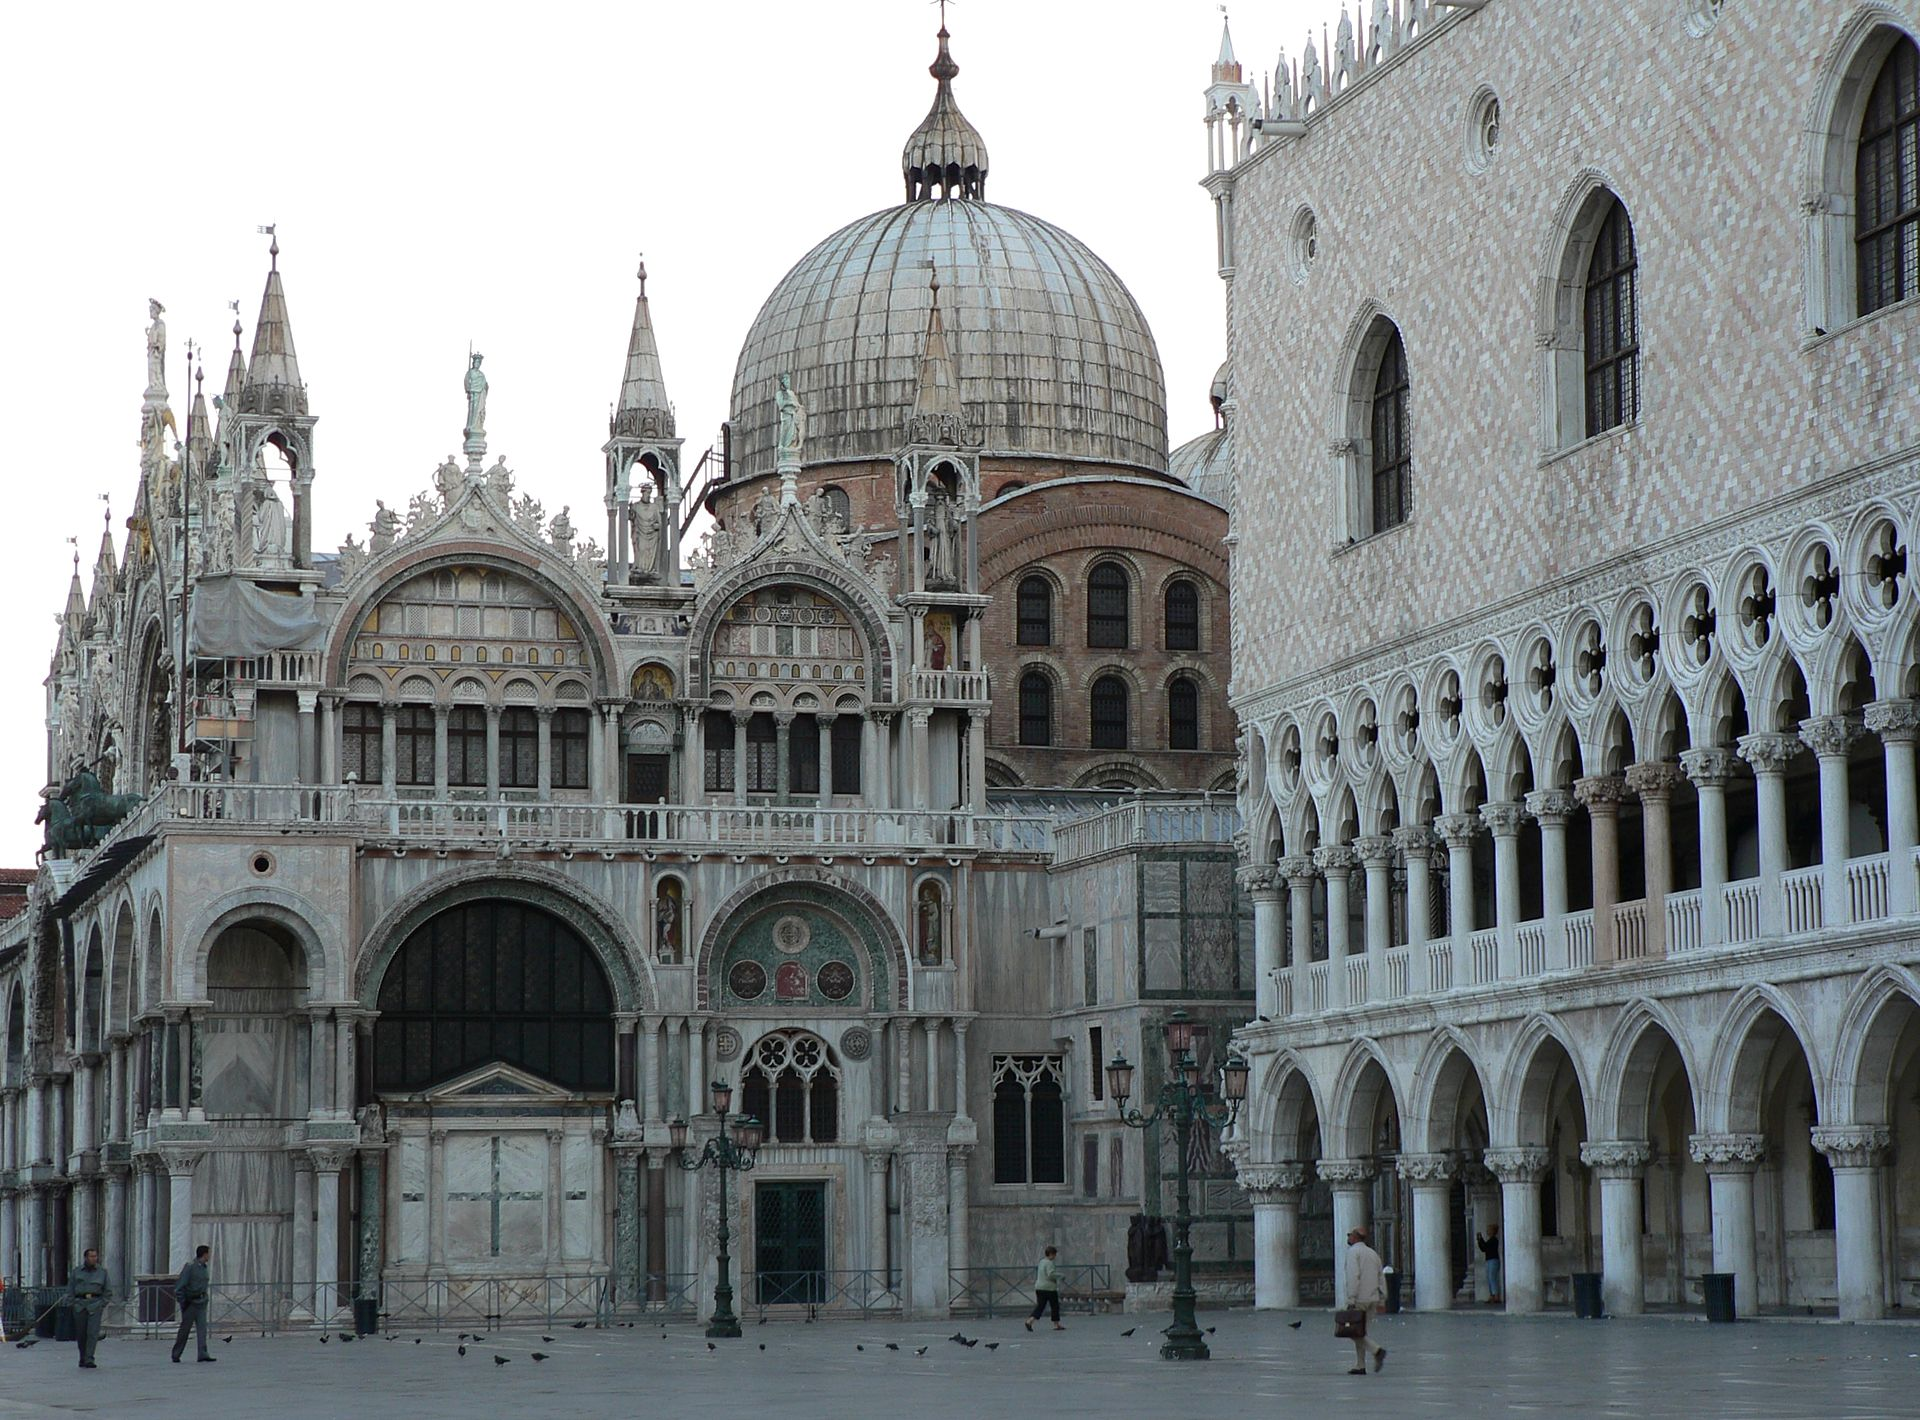
\includegraphics[width=0.7\textwidth]{img/basilica-san-marcos.JPG} 
%\captionsetup{justification=centering}
\caption{Basilica de San Marco \cite{Venbasil3:online}}
%license: cc by sa 3.0
\end{figure}

As a result of Willaert's work the practice of spatial music quickly spread to other parts of Europe where it was quickly adopted by composers such as Thomas Tallis in England. \textit{Spem in alium}, one of Tallis's most famous pieces, was composed for Queen Elizabeth upon her 40th birthday, in 1573, and featured 40 vocal parts arranged in eight 5-voice choirs. The high point of spatial music during the baroque era might however be Orazio Benevoli's\footnote{Franco-Italian composer born in Rome (19 April 1605 – 17 June 1672).} \textit{Festival Mass}, written in 1628 for the \textit{Salzburg Cathedral} which called for 16 vocal parts, 34 instrumental parts, two organs, and a basso continuo\footnote{Figured bass where the most common combination is harpsichord and cello for chord and bass-line respectively.} \cite{zvonar1999history}.

Following the baroque era, interest in spatial music subsided until the beginning of the Romantic period. A key distinction of this era is the use of spatial music for theatrical effect. The romantic period is often characterized by the rise and popularity of operas by composers such as: Hector Berlioz, a French Romantic composer and conductor (11 December 1803 – 8 March 1869) who wrote \textit{Requiem} in 1837, and Gustav Mahler, an Austro-Bohemian Romantic composer (7 July 1860 – 18 May 1911)\footnote{Considered one of the leading conductors of his generation.} who wrote \textit{Symphony No.2} in 1895 \cite{einstein1948music}. These composers not only spaced instruments for their performances but also choreographed the entrance and exiting of musicians as they played, creating some iconic musical moments.

In the 20th century, experimentalists such as Charles Ives, American modernist composer (October 20, 1874 – May 19, 1954), and Luigi Russolo, Italian Futurist composer and the author of the manifesto \textit{The Art of Noises} (30 April 1885 – 6 February 1947), inspired by the tumultuousness of industrial life, refined the art of musical collage using spatial sound \cite{jones199120th}. Ives's 1908 \textit{The Unanswered Question} called for offstage strings. Charles was inspired by his father George, a Civil War bandmaster, and music teacher, who had himself experimented with spatial music in his days. 

Henry Brant\footnote{Canadian-born American composer whom composed numerous orchestral spatial works (September 15, 1913 – April 26, 2008).}, inspired by Ives's music, would go on to create \textit{Antiphony I} (1953) which called for five spatially separated orchestras, and, \textit{Voyage Four} (1963) which called for three conductors to direct: percussion and brass on stage, violins on one balcony, violas and celli on another, basses on the floor level at rear, woodwinds at a rear balcony, and several performers in the audience \cite{zvonar1999history}. Brant's \textit{Windjammer} (1969), likely inspired by the opera composers of the baroque times, featured a static horn soloist and several wind players that moved along prescribed routes as they performed, in a choreographed manner. 

\cite{harley1997american} provides a rich analysis of four of Brant's most important works in the field of spatial music. Brant emphasized the need for differing timbres to be represented in his music, since he believed the heterogeneity would aid in the clarity of the musical representation. Indeed, if multiple instruments of the same family were spatially distributed, it would be difficult to differentiate melodic phrases, especially if these were all playing in the same register. 

% Brant summarized his main observations with regards to spatial composition in a 1967 articles paraphrased as following: 
% \begin{enumerate}
%     \item \textbf{Spatial separation clarifies texture}: when multiple musicians play different musical phrases in the same octave range, separating them spatially helps give clarity to each stream. 
%     \item \textbf{Separate groups are difficult to coordinate}: exact rhythms might be difficult to accomplish due to the distance it takes for sounds to arrive from one playing position to the next. 
%     \item \textbf{Spatial separation is equivalent to range separation}: it is possible to enhance the texture of a melodic phrase simply my separating musicians playing the same material.  
%     \item \textbf{Spatial arrangements must allow flexibility}: the specific architectural demands of the works cannot always be met, alternatives should be provided whenever possible.
% \end{enumerate}

Brant is perhaps one of the mos prolific composers of spatial acoustic works with a repertoire of 67 spatial pieces. Brant also wrote extensively on the subject of spatial music and experimented at length with form, rhythm and perceptual experience in this context. In contrast to other composers of his era, Brant's music dealt exclusively with acoustic means, which he creatively articulated to provide depth, envelopment and movement.  

\todo[inline]{There are still more works by Brant that might warrant mentioning.}

\subsection{Electro-acoustic Music} \label{subsec:elec_acoustic_mus}

Along a parallel branch of history there exist a number of musical experiments conducted in the 20th century by avant-garde musicians and composers typically categorized as \textit{electro-acoustical}. This label is used to separate them from traditional composers who avoided electronics or seldom exploited electronics in their compositions. The composers of this space and time were all activated by the development of sound recording, radio and telephony, and used them purposefully in their works. With the possibility of sound as a medium displaced from its source, dozens of new forms of music were created.

The birth of recorded sound brought along an era of technological music development featuring composers and engineers striving to encourage audiences to attend live events. Thaddeus Cahill's (1900-1906) \textit{Telharmonium} (1897) is considered the first electrical musical instrument of its kind \cite{bode1984history}. Also known as the Dynamophone, this electrical organ, which employed additive synthesis, was used to deliver music to homes on a subscription basis via a telephone line. We should note here that the element of space is present in an example such as this one, in a different semantic context, given the distance created between performer and audience. This device was in part inspired by Clement Ader's \textit{Théâtrophone} (1881), which sent stereo signals of actors via telephone wires \cite{TheTelh3:online}.

\begin{figure}[ht!]%force figure here, top, strict
\centering
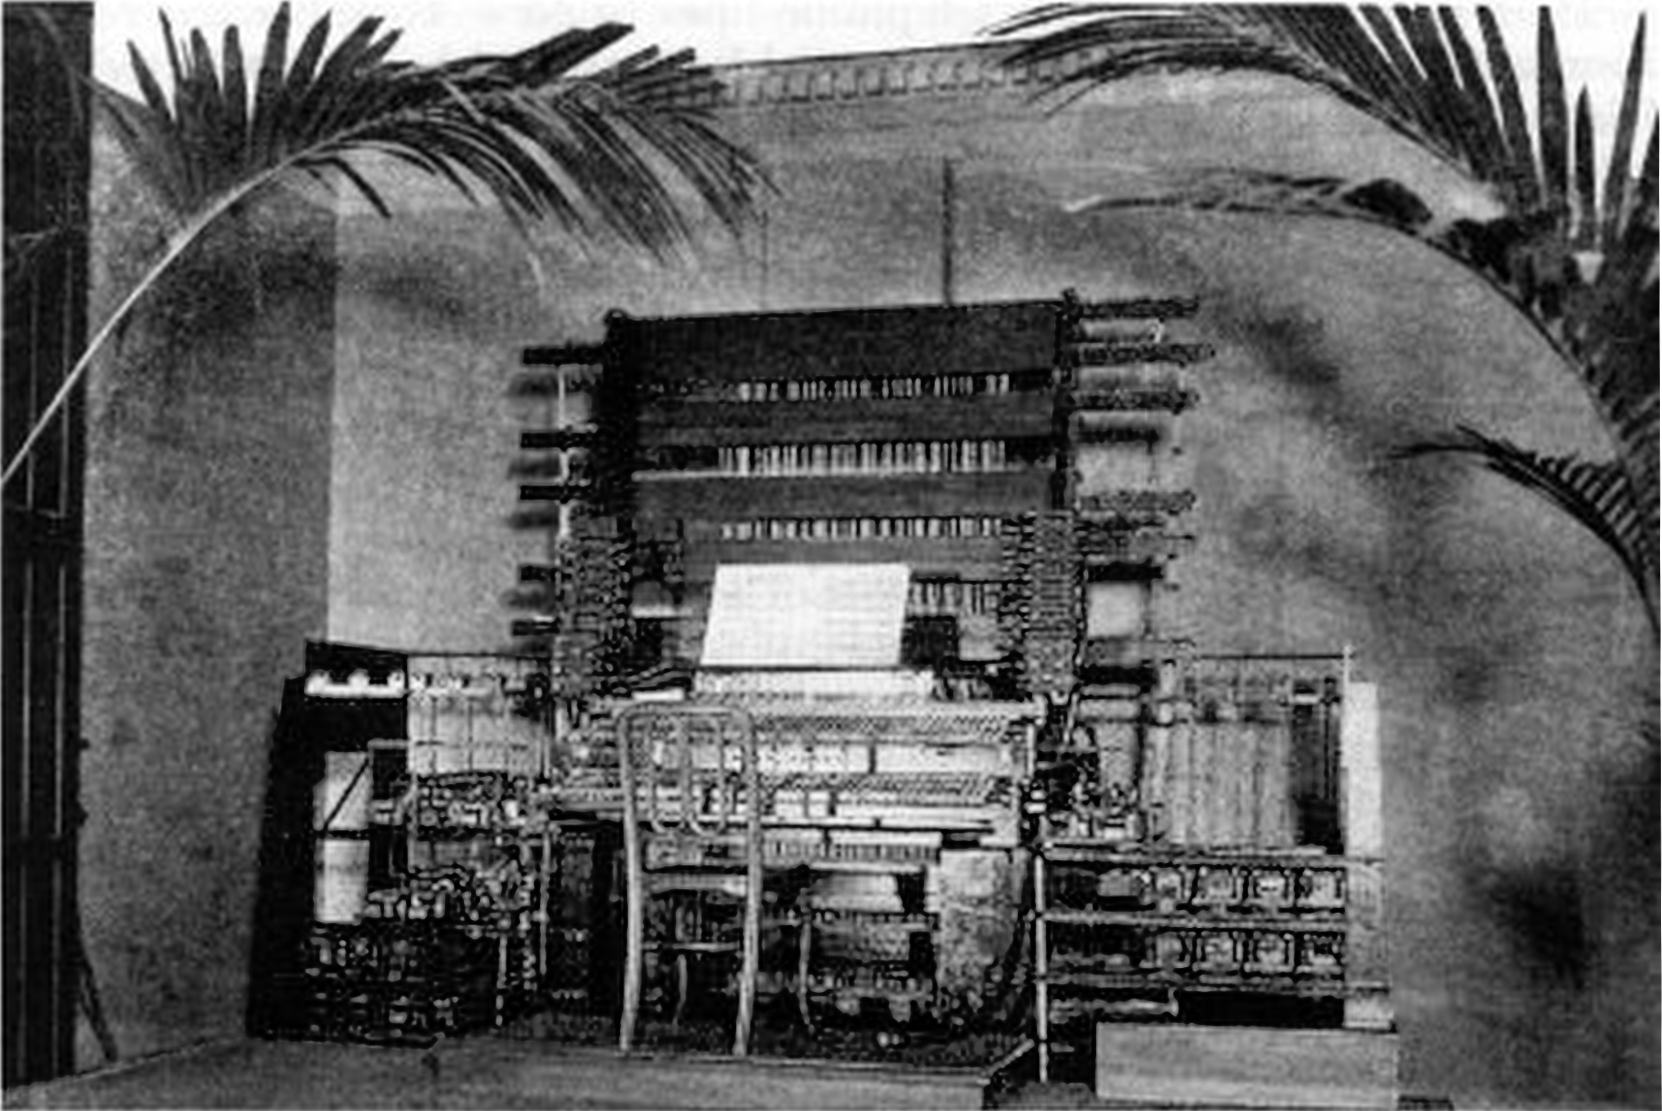
\includegraphics[width=0.8\textwidth]{img/telharmonium.jpg} 
%\captionsetup{justification=centering}
\caption{Telharmonium \cite{Telharmo82:online}}
%license: public domain
\end{figure}

Later, in 1923, Leon Theremin would introduce a new instrument to the public. The \textit{theremin}, named after its inventor, used two antennae to control the pitch and volume of a synthesizer. The user must position their hands in space to control the instrument and produce the desired sound. Theremin later formed ensembles in which multiple theremin were used in one of the first public displays of multi-channel loudspeaker music ever. The theremin is another particularly provoking example as it illustrates not only how space can be used for acoustic effect, but ergonomically speaking, it shows how an instrument can use space to facilitate its playing. Neither of these two instruments, however, exploit psycho-acoustic principles, the development of such instrument would come later. %spatial instrument

\begin{figure}[h!]%force figure here, strict
\centering
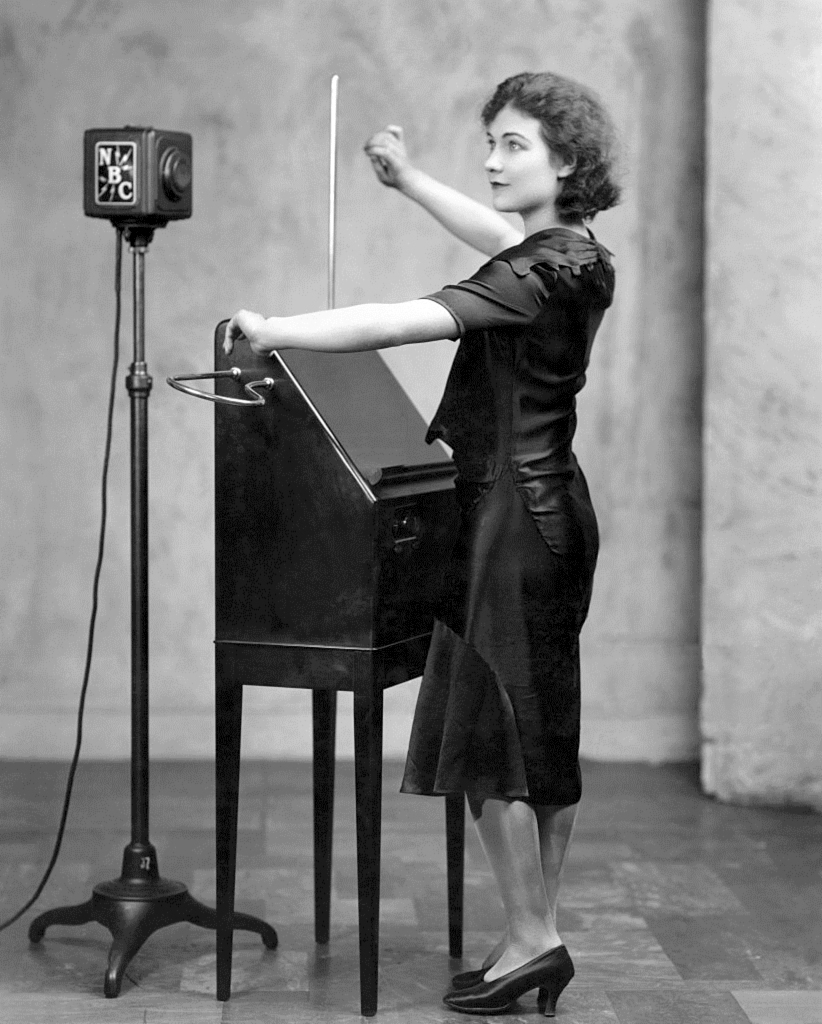
\includegraphics[width=0.5\textwidth]{img/theremin.jpg} 
%\captionsetup{justification=centering}
\caption{Alexandra Stepanoff\protect\footnotemark playing the theremin on NBC Radio, 1930 \cite{Theramin45:online}}
\end{figure}

\footnotetext{Alexandra Stepanoff was one of Léon Théremin’s first theremin students in the United States \cite{2020_stepanoff}.}

The 20th century also saw the rise of phonographs\footnote{Colloquially known as record players.} as musical instruments. Paul Hindemith\footnote{Prolific German composer (16 November 1895 – 28 December 1963).} began this practice in the 1920's and 30's nearly 80 years before DJing practices became popular \cite{manning2013electronic}! John Cage\footnote{American avant-garde composer (September 5, 1912 – August 12, 1992).} also adopted the use of phonographs compositionally in \textit{Imaginary Landscape No. 1} (1939) which used multiple turntables and test tones, and in \textit{Imaginary Landscape No. 4} (1951) where he used 12 radios, 24 performers and a conductor. In addition to exploring the use of phonographs as instruments, Cage also exploited radio broadcast and tape in his creative practice.  

By separating the original performer from the playback these composers were playing not just with space, but also time. Cage, along with a group of experimental composers called "Project for Music for Magnetic Tape", would go on to write four pieces for tape \cite{cage1961experimental} during the 50s. The most famous piece that emerged from the group was likely \textit{Williams Mix}\footnote{\href{http://tre.ucsd.edu/wordpress/?p=644}{Tom Erbe created a Pd version of William's Mix. (access: Jan 7, 2021)} } (1952) which called for 8 tape machines each played back from its own speaker and hundreds of sounds carefully spliced together. This was one of Cage's first use of chance in musical composition. The project also resulted in works by Earle Brown\footnote{American composer who pioneered the use of graphic scores (December 26, 1926 – July 2, 2002).} (\textit{Octet}) and Morton Feldman\footnote{American composer perhaps best known for his extended works which could last up to six hours (January 12, 1926 – September 3, 1987).} (\textit{Intersection}), both using 8 tape players and speakers. 

\begin{figure}[ht!]%force figure here, top, strict
\centering
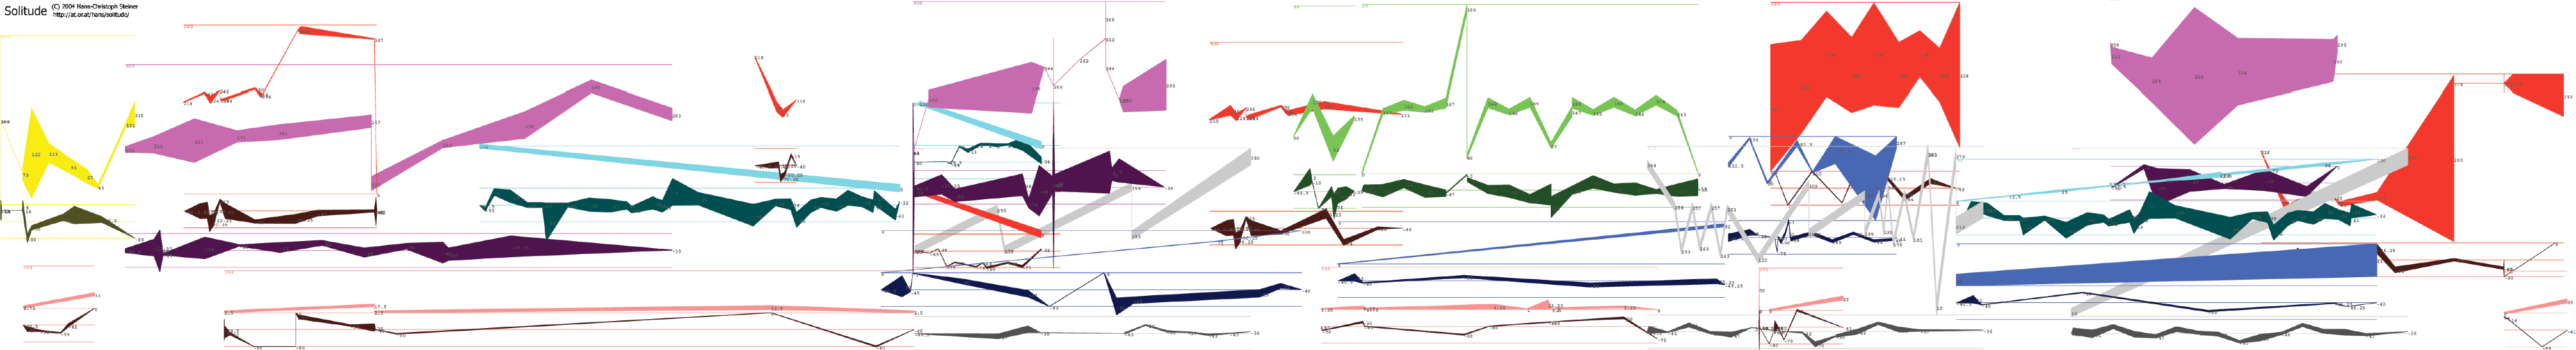
\includegraphics[width=1.0\textwidth]{img/solitude.png} 
%\captionsetup{justification=centering}
\caption{Hans-Christoph Steiner's\protect\footnotemark graphic score for Solitude, created using Pure Data's data structures. An example of a graphic score, such as those popularized by Earle Brown. \cite{wikipedia_2020_graphic}}
\end{figure}

\footnotetext{\href{https://at.or.at/}{Hans-Christoph Steiner's site.}}

Cage, Brown and Feldman were greatly influenced by Pierre Schaeffer, a french engineer at Radiodiffusion-Television Francaise (RTF), who in 1948, presented the first musical works created with disk recorders. These were the first examples of \textit{musique concrète}, a style of music which is defined by the use of recorded sounds interpreted as musical material. Schaeffer would later go on to collaborate with Pierre Henry, another notorious French composer, creating a repertoire of works for tape including, most notably \textit{Symphonie pour un Homme Seul}, which translates to "Symphony for one man alone". (1950). 

In their 1950 piece, four channels were arranged in a tetrahedral\footnote{Three sided pyramid.} configuration with two front speakers, one back speaker, and a final overhead speaker, making this one of the first examples of \textit{periphonic}\footnote{Periphonic refers to sound with height, while \textit{pantophonic} is used to denote sound systems with horizontal-only reproduction.} music. Schaeffer also helped developed the \textit{potentiomètre d'espace}, one of the first \textit{spatial audio} audio controllers which he controlled during live performances to modify the amplitude of speaker feeds. 

In Germany, another composer by the name of Karlheinz Stockhausen was making his mark in \textit{electro-acoustic} music. Stockhausen is perhaps the most ambitious composer of \textit{spatial music} in this era. Inspired by tape music, Stockhausen would travel to RTF, the birthplace of tape-based works, to learn about the technology. Soon after his time at RTF, he would return to Westdeutsche Rundfunk's (WDR) Studio fur Elektronische Musk\footnote{Which translates to studio for electronic music.} to create his most prolific tape pieces. \textit{Gesang der Jünglinge}\footnote{Which translates to "Song of the Youths".} (1956) is considered by some as the first piece for multi-track tape, using a 4-track machine plus a fifth mono tape player for the fifth channel. The premiere featured a number of speakers arranged \textit{panoramically} onstage \cite{zvonar1999history}. Stockhausen later remixed this piece for quadraphonic sound\footnote{Playback system which uses 4 speakers.} system. In 1960, he would go on to create \textit{Kontakte}, his first truly quadraphonic piece. Stockhausen used a turntable system with a rotating speaker and four microphones to create the illusion of spinning sounds. Stockhausen also explored spatial attributes of sound in his acoustic compositions written for multiple orchestras and multiple choruses. His most ambitious and bizarre work is perhaps \textit{Helikopter-Streichquartett} (1993), completed much later. In this piece the four members of a string quartet perform from four helicopters, which fly independent routes, and each have their own audio-visual system, along with a sound engineer. The sound and video is transmitted to the concert hall. The sound from the flying helicopters is also part of the piece \cite{stockhausen1996helikopter}. 

In 1958, another one of the most important examples of spatial electronic music would be performed. Edgard Varèse's\footnote{French-born composer (December 22, 1883 – November 6, 1965). Varèse coined the term "sound mass" to describe his music.} \textit{Poème Électronique} was featured at the Brussels World Fair (Expo 58), a major international event with artists from all over the world. The festival attracted up to two million visitors! For the exposition of this piece, the Philips Corporation set up 15 tape recorder and over 400 loudspeakers \cite{malham19953}. This is still one of the largest spatial music compositions that have ever been accomplished. Xenakis, another giant of electro-acoustic music, designed the Philips Pavilion under the supervision of renowned Swiss-French architect Le Corbusier (1887-1965). Xenakis's \textit{Concret PH}, created using recordings of burning charcoal, modified using tape techniques, also played at the Expo, as an interlude between performances of Varèse's piece, which was the main attraction\cite{valle2010concrete}. Expo 58 also featured \textit{Vortex}, a series of thirteen programs developed by Jordan Belson and Henry Jacobs for the Morrison Planetarium in San Francisco. The program featured music by Stockhausen among many others \cite{zvonar1999history}.

\begin{figure}[h]%force figure here, top, strict
\centering
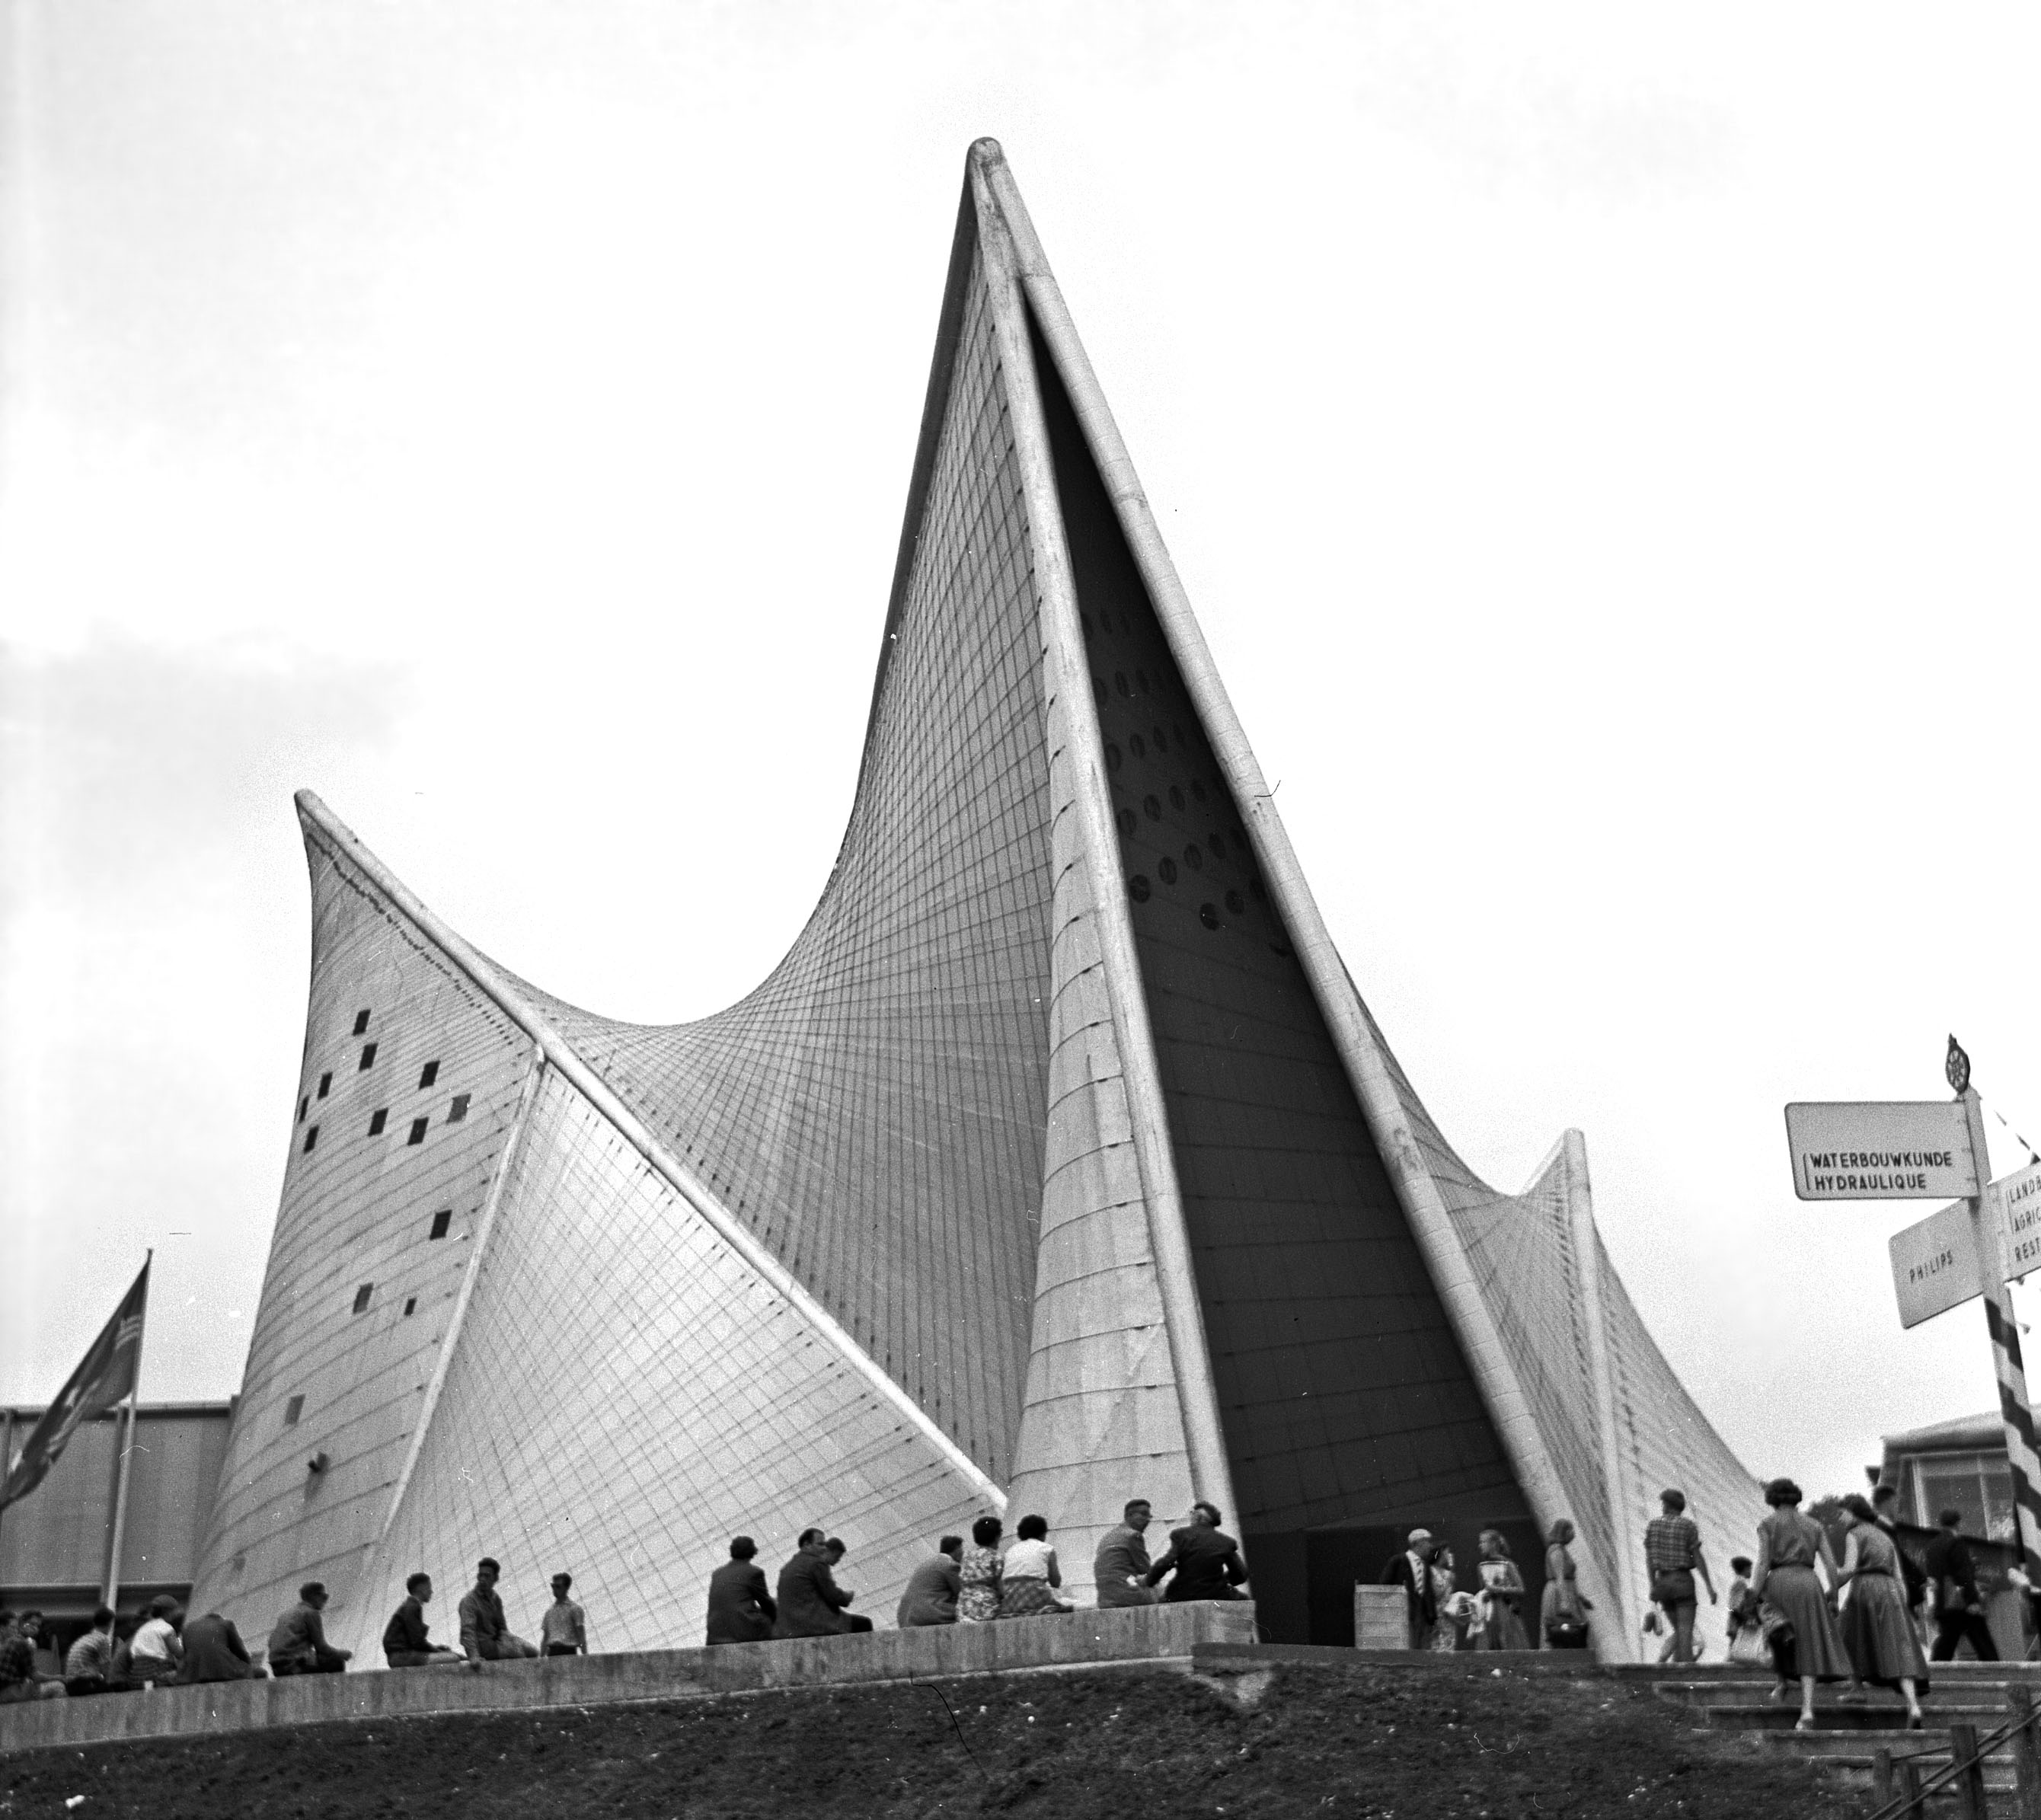
\includegraphics[width=0.5\textwidth]{img/expo58.jpg} 
%\captionsetup{justification=centering}
\caption{The Philips Pavilion \cite{wikipedia_2020_expo}}
\end{figure}

EXPO 70 in Osaka, Japan, also featured a number of groundbreaking spatial works. There, Xenakis presented a 12-channel tape composition titled \textit{Hibiki Hana Ma}, which translates to "Reverberation Flower Interval", was composed using the UPIC system. The UPIC\footnote{Unité Polyagogique Informatique CEMAMu (Centre d'Etudes de Mathématique et Automatique Musicales).} system was an instrument which allowed the composer to draw scores which would be interpreted by a machine\footnote{The software \href{https://www.iannix.org/en/whatisiannix/}{iannix} is the modern equivalent of the UPIC system.}. The graphical input device was used in conjunction with orchestral recordings, biwa\footnote{Japanese plucked instrument resembling a lute or guitar.} recordings, and snare drum recordings \cite{IannisXe73:online}. For the performance at the Japanese Steel Pavilion the sound system featured 800 speakers situated above, around, and even under the seats. At the same time, in the German Pavilion, Stockhausen, along with 20 soloists, were performing in a spherical auditorium featuring 55 speakers and six small balconies. The auditorium had an acoustically transparent grid which allowed sound to emanate from below the seating area which seated 600 people \cite{zvonar1999history}.

\begin{figure}[h]%force figure here, top, strict
\centering
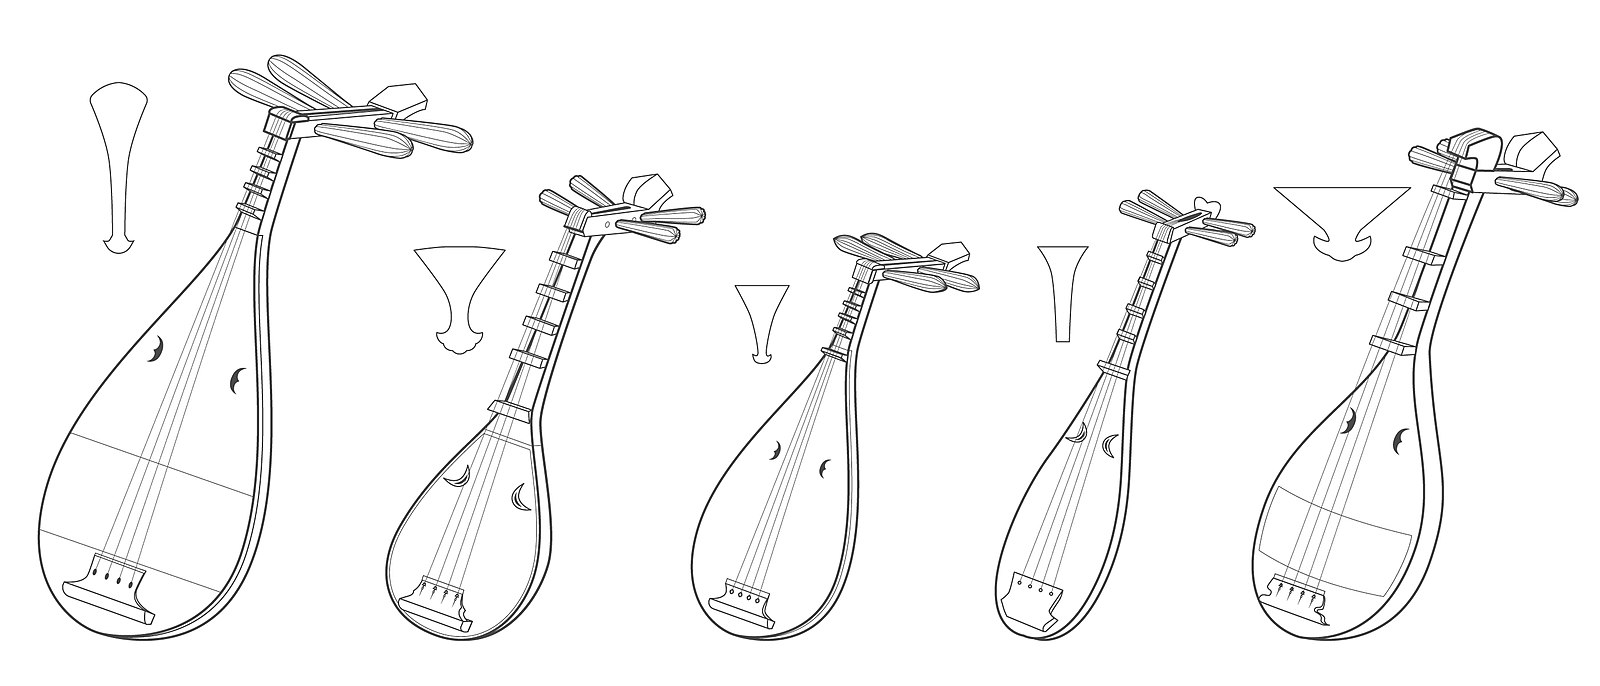
\includegraphics[width=0.7\textwidth]{img/types-of-biwa.jpg}
%\captionsetup{justification=centering}
\caption{Types of Biwa \cite{FileType46:online}}
%license: attribution share alike 4.0
\end{figure}

The Pepsi Cola Pavilion was another space created for EXPO 70 - this time designed by an American group called: "Experiments in Art and Technology" (EAT). The domes' 37 loudspeakers were arranged in a rhombus and could be driven with 16 monaural tape recorders and 16 microphone preamps for a total of 32 inputs. There were also 8 signal processing channels with amplitude modulation (AM), frequency modulation (FM) and various filters, which these sources could be routed to. Handsets were also distributed which could pick up sound in each of 11 zones. The dome was outfitted with laser beams and fog machines, and the walls of the dome itself were made of specular surfaces, for added dramatic effect. The dome was designed as a modular instrument, which could be reconfigured to fit the range of artists' visions \cite{bertrand2012pepsi}.

Given the wide range of creative options for spatialization of sound \cite{zvonar2000extremely} provides a list of the different types of electro-acoustic works in relation to their associated techniques - along with some influential composers representative of each method - to help us understand their differences:

\begin{enumerate}
    \item Live performance or "diffusion" of sound (Pierre Henry).
    \item Environmental multi-channel soundscape (John Cage).
    \item Classic studio multi-track tape composition (Karlheinz Stockhausen).
    \item Automated location control (Edgard Varèse).
\end{enumerate}

In this "live performance" setting, Pierre Henry created a repertoire of tape works which would be \textit{panned} around in real-time according to the desired trajectories manipulated by the composer. These works made use of Schaeffer's aforementioned \textit{Potentiometre d'espace} created in 1951, which translates to spatial potentiometer\footnote{A potentiometer is an electrical component which allows one to manually change the resistance between two points in a circuit.}. Henry also worked on diffusion works where stereo tapes would be played back over large loudspeaker systems. Examples of Cage's environmental works include \textit{HPSCHD}\footnote{Short for harpsichord. In collaboration with Lejaren Hiller, another American composer.}(1960) which used 58 channels - seven for harpischord soloists and 51 for computer generated tapes. The result of all this sound sources was a dense microtonal sound mass. There were also 80 slide projectors, seven film projectors, and a 340-foot circular screen. The piece was 5 hours in duration, however, participants were encouraged to enter and leave the environment as they desired. The final two classifications refer to works which are: "fixed" - suggesting that the trajectories of sounds are imprinted into the tapes and never controlled during the performance - and, those which use an algorithm\footnote{In Varèse's case the algorithm was imprinted on tape.} to manipulate the real-time diffusion\footnote{Diffusion in this context meaning panning of sound sources in space.} of sound sources. 

David Tudor was another member of John Cage's group who developed a series of installations of similar nature. \textit{Rainforest} (1968) is his best known work. In this installation work speakers are placed inside objects in order to activate their resonant modes. The sounds are consequently picked up using contact microphones, after they have been altered by the cavities of these objects. In Tudor's work, there were usually 4 to 8 speakers, but because of the additional resonant objects, the total speaker count was generally higher. Alvin Lucier, famous for the acoustic feedback composition: "I Am Sitting in a Room" (1969), explored a similar concept using the resonant modes of a room to create his piece. While not psycho-acoustic in nature, we can consider Lucier's piece a sort of architecturally spatial piece, dictated in large part by the geography and environment.

John Chowning, famous for his discovery of frequency modulation (FM), as a musical technique, at Stanford, also published and composed spatial pieces still relevant today. "The Simulation of Moving Sound Sources" \cite{chowning1971simulation}, published by Chowning in 1971, is considered a seminal piece of technical literature by a pioneering computer musician detailing his spatial audio algorithms. Chowning describes a system for the synthesis of spatial sound relying on FM and reverb to describe moving sources. FM in this context was used to simulate \textit{Doppler shift}. His piece \textit{Turenas} (1972), which makes use of a quadraphonic layout and this algorithm, was composed at CCRMA\footnote{Center for Computer Research in Music and Acoustics (CCRMA) at Stanford is an important computer music research facility.}, an important institution he was a founding member of. It should be noted here that the substantial difference in speaker count between \textit{Poème Électronique} and \textit{Turenas} had no impact on the historical importance of these works. It is easy to believe that higher speaker count is crucial for great spatial music - Chowning's work demonstrates that this is not always the case.

Part of the reason for the lower speaker count in some of these early works can be explained by the exorbitant cost of computers capable of handling these processes at the time. In 1981 at IRCAM\footnote{Institut de Recherche et Coordination Acoustique/Musique. Or, Institue for Research and Coordination Acoustical/Musical. It is organizationally linked to the Centre Pompidou in Paris.} the 4X synthesizer used to perform Pierre Boulez's\footnote{French composer perhaps best known for his large orchestral works featuring live electronics (26 March 1925 – 5 January 2016). Founding member of the aforementioned IRCAM.} \textit{Répons} (1985) had a cost of \$100,000. Today it is possible to recreate the synthesized elements of this piece using a personal computer \cite{zvonar2000extremely}. 

\begin{figure}[ht!]%force figure here, top, strict
\centering
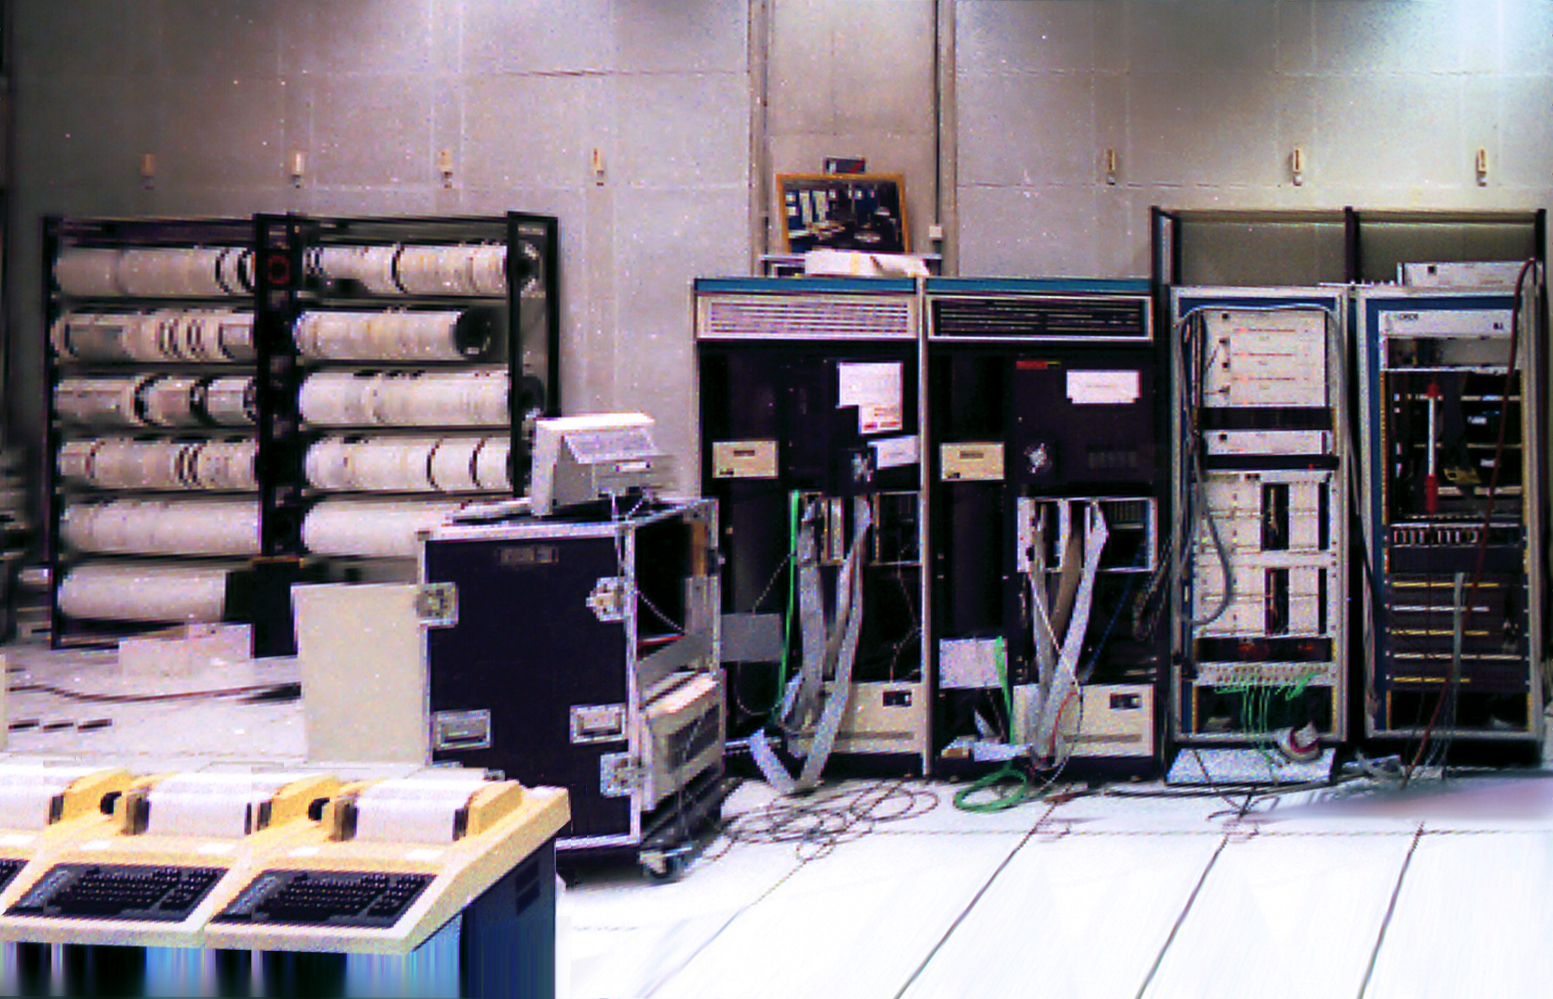
\includegraphics[width=0.7\textwidth]{img/ircam-4x.jpg} 
%\captionsetup{justification=centering}
\caption{IRCAM 4X \cite{FileIRCA45online}}
%  Creative Commons ShareAlike 1.0
\end{figure}

% \todo[inline]{Where can we find a patch for Repons? Is there a Pd port?}

Roger Reynolds in the 70s also created a number of important works. Reynolds used voice recordings in his \textit{Voicespace} pieces such as \textit{Still} (1975) and \textit{Eclipse (Voicespace III)} (1979). The pieces were created using analog equipment including: recorders, mixers, reverbs, and voltage controlled spatial location systems. \textit{The Palace (Voicespace IV)} (1980), used quadraphonic sound system and recording of singer Philip Larson, which were analyzed and processed to emphasize the harmonic content. A reverberation algorithm also gave the illusion of an impossibly huge space \cite{zvonar1999history}. Reynold's continued working with sound analysis in \textit{Transfigured Wind II} (1984). The piece features quadraphonic tape, solo flute and orchestra. There is also analysis and resynthesis of the flute using software created by IRCAM. \textit{Watershed IV} (1996), for solo percussion and computer is another example of his spatial works, this time featuring 6 speakers on stage and 2 additional surround speakers. The piece was performed by Steve Schick (1954), American percussionist and conductor. \textit{The Red Act Arias} (1997), another work by Reynolds, is based on the Greek tragedy of Clymenestra and Agamemnon. The piece features orchestra, chorus, and octophonic processed sounds using the \textsc{cmusic} "space" unit generator. \textsc{cmusic} was developed in 1980 by Richard Moore at the Computer Audio Research Laboratory (CARL) of the Center for Music Experiment at the University of California at San Diego (UCSD) \cite{moore1982computer}. \textit{Justice} (2000), by Reynolds, featured soprano, actress, percussionist, tape and computer spatialization. 

In Montreal in 1999, ACREQ\footnote{\href{https://www.thecanadianencyclopedia.ca/en/article/acreq-emc}{Association pour la Création et la Recherche Electroacoustiques du Québec}. The first non university-affiliated organization in Canada exclusively dedicated to electro-acoustic music.} reproduced Pierre Henry's \textit{L'Apocalypse de Jean} (1968) through a 24.6 sound system using the commercial CD as the sound source. Henry is one of the pioneers of this \textit{diffusion} practice, in which mono or stereo signals are played back over a multitude of speakers. Sound systems such as the ones proposed by Henry are sometimes referred to as an \textit{acousmonia}\footnote{Acousmonium being the singular.}. Here the sound system becomes and instrument itself, to be performed by the composer using, traditionally, musique concrète. François Bayle designed the first acousmonium in 1974 which was used by Groupe de Recherches Musicales (GRM)\footnote{Institute created by Pierre Schaeffer in 1958 in France.}. The Gmebaphone and Cybernéphone at the Institut International de Musique Eléctroacoustique de Bourges (IMEB)\footnote{Central France.}, and the Birmingham\footnote{Second largest city in England.} ElectroAcoustic Sound Theatre (BEAST) are a few other examples. Notable American acousmonia include composer Stan Shaff's \textit{Audium: A Theatre of Sound-Sculpted Space} and the Recombinant Media Lab both in San Francisco. These are all historical examples of multi-channel sound systems, since then several institutions have developed their own diffusion systems for spatial music performance. These historically relevant systems have also evolved over the years from diffusion systems to arrays supporting modern spatialization algorithms.

\begin{figure}[ht!]%force figure here, top, strict
\centering
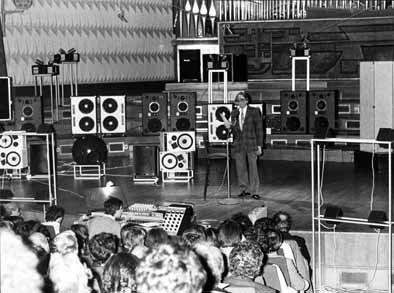
\includegraphics[width=0.7\textwidth]{img/acousmonium.jpg} 
%\captionsetup{justification=centering}
\caption{Pierre Schaeffer Presenting the Acousmonium \cite{FilePsco51online}}
% This file is licensed under the Creative Commons Attribution-Share Alike 3.0 Unported license.
\end{figure}

Denis Smalley is another pioneering composer who has worked, and continues to work, extensively with space in his acousmatic compositions. Smalley has created his own language to describe sound which he describes as spectromorphological. Has Smalley puts it in \cite{smalley1997spectromorphology}:

\begin{quote}
    Spectromorphology is not a compositional theory or method, but a descriptive tool based on aural perception. [...] Although spectromorphology is not a compositional theory, it can influence compositional methods since once the composer becomes conscious of concepts and words to diagnose and describe, then compositional thinking can be influenced, as I am sure my own composing has been.
\end{quote}

Smalley has created an extensive dictionary to describe the way he envisions and articulates his music. \cite{blackburn2011visual} pictorialized some of these concepts in order to help the reader better understand Smalley's language. Here we will only present written definitions of some of the most popular concepts defined by Smalley. 

\begin{enumerate}
    \item \textbf{Source-bonded space:} refers to the spatial zones and mental images produced by, or inferred from, sounding sources, and their causes (if there are any). 
    \item \textbf{Source bonding:} related to source-bonded space, is the \textit{natural} tendency to relate sounds to \textit{supposed} sources and causes, and to relate sounds to each other because they appear to have shared or associate origins.
    \item \textbf{Perspectival space:}  relating to our perspective, can be further sub-divided into various perspectives.
    \begin{enumerate}
        \item \textbf{Prospective space:} frontal image, which extends to create panoramic space.
        \item \textbf{Panoramic space:} the breadth of the prospective space, extending the limits of the listener's peripheral view.
        \item \textbf{Circumspace:} the extension of prospective/panoramic space so that sound can move around, above and through the space occupied by the listener.
    \end{enumerate}
    \item \textbf{Spectral spatiality:} impression of space and spaciousness evoked by occupancy and motion within the range of audible frequencies.
\end{enumerate}

This list forms only a small part of the language created by Smalley to describe his music. \textit{Pentes} (1974), \textit{Empty Vessels} (1997), \textit{Wind Chimes} (1987) and \textit{Valley Flow} (1991–92), are a few of Smalley's most notorious compositions in which he attempts to sonically articulate all these different concepts. \cite{o2011soundscape} provides a closer examination of these works. According to O'Callaghan, many of Smalley's works utilize mimetic properties. In other words, the sound design aims to simulate real world sounds using electro-acoustic means. Much like work done by Barry Truax such as \textit{Riverrun} (1986) which utilizes granular synthesis to emulate the sound of a flowing river.

This brings us to the conclusion look into the history of spatial music. As we can see, while many contemporary composers might attribute the development of spatial music to composers of the 20th century, the use of spatial elements in composition has a longstanding tradition that spans hundreds of years. 

\todo[inline]{ macedo-2015-snd-in-space.pdf} 

\section{Installation works}

In this section we wish to enumerate some of the \textit{sound artists} whom have created interesting and powerful spatial music works in their practices. In contrast to concert events, these installation pieces are designed to be shown in art galleries and experienced by hundreds of people over many days. 

Michael Asher (July 15, 1943 – October 15, 2012), the first in our list, was a conceptual artist who worked with sound absorption and acoustic phase cancellation in his works. In \textit{Spaces} (1969), Asher created a sonic space which resulted in different aural experiences as one walked around the gallery. Michael Brewster also worked with these ideas as well as: room resonances, standing waves, and acoustic shadows. Both of these artists sought to manipulate air as a sculptural medium. Some of Brewster's most famous works include \textit{allAROUNDyou} (1998), \textit{See Hear Now} (2001) and \textit{full o’stuff} (2000) \cite{macedo2015investigating}. 

Maryamme Amacher is one of the most ambitious and well-known artists of sound art employing spatial elements. Her work explored structural vibrations and structure-borne sound. In \textit{Music for Sound-Joined Rooms} (1980) she transformed an old house into a resonator by placing powerful speakers inside it. In \textit{City Links} (1967-80) she installed microphones at the Buffalo Airport and Boston Harbour and connected the spaces sonically with speakers. Listeners in Buffalo heard the sound of the Harbour, while people in Boston heard the sounds of the airport. Amacher also created CDs with music specifically meant for loudspeaker reproduction. She believed the physical characteristics of the listeners space was instrumental in appreciating her work\cite{ouzounian2008sound}. Amacher is also known for exploring sonic relationships with \textit{otoacoustic emission} in her work. Otoacoustic emission refers to sound that originate from the inner ear, in some people it manifests as a medical nuisance called \textit{tinnitus} \cite{brummer2017composition}.  

Edwin van der Heide, a Dutch sound artist, also explored architectural interactions with sound in \textit{Speed of Sound} (2007). The piece explores the effects of four corridors in the shape of rings on sound. As Heide puts it in \cite{TheSpeed60online}:

\begin{quote}
    "The propagation of sound in the rings of the water reservoir of Prenzlauerberg in Berlin is the starting point for the installation. The acoustic sound in the space is being picked up, transformed and re-entered in the space. The transformations, delays and spatial interconnections are part of a time based process that can be seen as a composition for the environment."
\end{quote}

Similarly, in \textit{Crescents} (2010) Raviv Ganchrow explores the reverberance and general acoustic character of spherical domes in Estonia. In this example the acoustic space is central to the work, and the variability from moment to moment is created by the dynamic architectural features. However, there are also sound artists who have explored spatialization in their works. 

In two of his \textit{Three Sounds} (1971) Howard Jones explored the motion of sound \cite{macedo2015investigating}. In \textit{Linear Relay} a metronome sound is played through 20 speakers all aligned in different ways. \textit{Area Relay} also explores this idea by using 9 speakers assembled in a grid playing different sounds to provide the illusion of distance and depth. Bernard Leitner's installation \textit{Sound Space} (Berlin, 1984) used 48 speakers hidden behind panels in the walls of a staircase to simulate trajectories.  

\textit{Sound Island} (1994) by Bill Fontana, an American sound artist, used 48 speakers across the Arc de Triomphe in the centre of Paris to receive and reproduce sounds from the coast of Normandy. There is also Max Eastley's \textit{Sutton Edge} (1991) in which Max installed a set of ad hoc wind harps in an open site \cite{ray2006soundscapes}. William Louis Sorensen explored a similar idea in \textit{Landing Ground for Waders} (1983) using more humble materials such as wine bottles, wood and plastic. 

Two other related examples are Westerkamp's \textit{soundwalks}, in which listeners are simply asked to traverse any environment with the main purpose of listening, and Steve Peters’s \textit{Here-ings} which are collections of recordings in central Mexico, meant to transport the listener to the space\footnote{https://www.spsoundart.com/hereings}. 

A final sound art work we sought to include is Alvin Curran's 1987 \textit{Notes from the Underground}. The work was part of a larger collection titled Music from the Center of the Earth, however the rest of the remaining works never seem to have been realized, they only exist in concept. In \textit{Notes from the Underground} the idea was to create sound walls by physically burying speakers underground. Its realization was commissioned by the Ars Electronica Festival\footnote{A prestigious media arts festival in Lintz, Austria.} in 1991. The collaborator in the project, Mellisa Gould, used the floor plans of an old Berlin synagogue for this Holocaust memorial. The music was composed a Mills College's Center for Contemporary Music, in Oakland, California. Then the tapes were used to drive 72 speakers in groups of 8 attached to 9 stereo amplifiers\cite{curran1994music}\footnote{The system was designed by Tom Erbe who studied at Mill's College at the time.}

\todo[inline]{xenakis "polytopes"}
% https://www.theguardian.com/music/tomserviceblog/2013/apr/23/contemporary-music-guide-xenakis

% iannix graphic score editor

\section{Contemporary Spatial Music} \label{sec:contemp_works}

Several authors have explored the use of space in composition with varying degrees of success. In this section we will explore the techniques and aesthetics employed by these composers. The following pieces in this section were selected because the composers all use "spatial articulation as a central element in the musical construction\footnote{Lyon in Sound Anthology Program Notes CMJ 41:1}". Our hope is that by understanding the methods and processes used by some of these composers the reader might be better equipped to create impactful spatial music and carve their own style to differentiate themselves from the many other artists in this field.

\subsection{Concert music}

\cite{hagan2017sound} offers an overview of some of the current leading figures in the development of spatial music. Before diving into the particular composers and their works two noteworthy facts stand out from these program notes. The first interesting information is that the delivery of the musical material\footnote{Found \href{https://muse.jhu.edu/article/656037}{here}. Jump to end of page to download audio files.} for public consumption used a stereo format with binaural properties. What this means is that the music does have spatial attributes, but much of it will be lost because the listener will not have the ability to rotate the soundfield in relation to their head orientation. The second noteworthy piece of information is that in this anthology Hagan and Lopez-Lezcano opted for \textit{static binaural synthesis} while the rest create binaural recordings - using a dummy head. This offers the listener the possibility, albeit with different materials, to experience the quality changes between both spatial audio rendering methods.

We will discuss the different composers in order of appearance within the program notes. \textit{Spin} (2016) by Ludger Brümmer was created by taking video files and converting these into noisy sound material. The sound is then organized contrapuntally and the resulting soundfield is spun over the course of the piece. This piece was recorded at the \href{https://zkm.de/en}{ZKM Klangdom} in Germany using 32 channels. \cite{ramakrishnan2006zkm} provides a rich description of the "Kubus" which is the name of the concert hall where this piece was recorded. \textit{Spin} has a very synthetic quality to it and resembles the score someone might hear in a sci-fi film. It features noises one could qualify as other-wordly: warps, glitches and combed filters appear to be prominent. Ludger's former interests also include physical modeling and granular synthesis, both of which also appear to be exemplified here. 

\begin{figure}[ht!]%force figure here, top, strict
\centering
\includegraphics[width=0.7\textwidth]{img/zkm-commons.jpg} 
%\captionsetup{justification=centering}
\caption{ZKM - wikimedia commons}
\end{figure}

\textit{Sveti Kliment} (2007) by Robert Sazdov and was recorded at the Sonic Lab of the Sonic Arts Research Centre (SARC) in Belfast, Northern Ireland. The composition was inspired by Saint Clement of Ohrid from the Orthodox Church of Macedonia, a patron saint of education and language who committed his life to: research, teaching, and improving the lives of "those in his diocese". The piece open with the natural sound of a flute but quickly morphs into a soundscape of reversed noises and unintelligible speech snippets. The timbre of the flute reappears as a thematic motif and its reverberation is frozen and played over, using the same instrument. The timbre of the flute seems to be that of a ethnic instrument perhaps in reference to the Balkans. 
\cite{lynch2017perceptual}, co-authored by Sazdov, discusses some of the most popular and powerful spatialization techniques, used routinely by composers. In this paper, the author used four of these critical techniques in a subjective experiment in order to determine listener preferences. The techniques used in that experiment are described as follows:

\begin{itemize}
    \item \textbf{Timbre spatialization}: in this technique the source signal is copied and routed to multiple band-pass filters. These filtered versions of the original sound signal are sent to various speakers. The bandwidth of these filters can be modulated for artistic effect. 
    \item \textbf{Spectral splitting}: is a technique used in periphonic configurations, wherein the loudspeakers in the upper regions are assigned a high pass-filter in order to cut frequencies below a certain range. 
    \item \textbf{Amplitude point-source panning}: amplitude point-source panning consists of placing monophonic sound signals on individual loudspeakers. Perceived movement of sounds between loudspeakers is achieved by changing amplitude levels of individual speakers.
    \item \textbf{Dynamic spectral sub-band decorrelation}: similar to timbre spatialization but with modulated center frequency for band-pass filters and added decorrelation copy (at same speaker) created using modulating sample delays. 
\end{itemize}

In addition to these four common techniques, Sazdov lists authors who have experimented with granulation approaches to spatialization. More recently \cite{rossetti2020studying}, Rossetti proposed a HOA \textit{granular synthesis} system in which individual grains are spatialized using 7th order ambisonics. Curtis Roads, famous for his use of granular synthesis (GS) in composition describes it as:

\begin{quote}
    "a kind of synthesis based on grains, a microacoustic event with a duration near the threshold of human auditory perception normally presenting a duration between 20 and 400 msec. The grains, by definition, capture two perceptual dimensions: the time-domain and the frequency-domain information, and each grain has a waveform shaped by an amplitude envelope\footnote{Such as a Hanning window.}. The GS [system] is an automation process in which thousands of grains are combined over time, creating sound textures (clouds or masses) of different densities and frequency ranges." \cite{roads2004microsound} 
\end{quote}

Another related approach undertaken by Einbond \cite{einbond2017mapping} involves using descriptors of sound samples to dictate the spatialization. This approach involves two stages: analysis and re-synthesis. In the analysis stage, sound grains are created and organized in \textit{Euclidean space} using analysis processes such extraction of \textit{Mel Frequency Cepstrum Coefficients} (MFCCs)\footnote{MFCC is more or less the FFT of an FFT mapped to the Mel Scale. Cepstrum is an anagram for spectrum (a rearrangement of its letters). An full explanation of MFCC is outside the scope of this text, we refer the reader to \cite{terasawa2005perceptual}.} for example. Euclidean space can be defined as the fundamental space of classical geometry which includes standard 3D space with coordinate mapped by coordinate $(x, y, z)$. These grains can then be played back using \textit{concatenative synthesis} and spatially distributed based on their Euclidean coordinates. In the Pd environment we recommend William Brent's \cite{brent2010timbre} toolbox for timbre analysis. Concatenation is a process common to arrays, to concatenate two vector means to place one right after the other.

\textit{Morphons and Bions} (2011) by Kerry Hagan is a real-time Puredata composition which relies on noise synthesis and randomness. \cite{hagan2012aesthetic} provides a richer description of the work. As opposed to Sazdov's piece, all the sounds in this piece are synthesized in real-time. According to Hagan: 

\begin{quote}
    "Because the work is built on a substrate entirely made of noise, the piece is situated within certain philosophical and aesthetic issues surrounding noise, its use, and its definition."
\end{quote}

Indeed, a lot of discussion has gone into the role of noise in contemporary music. Despite the abundance of noise in \textit{Morphons and Bions}, Hagan does not consider the piece to fall under the category of "noise music", given the harmonic and quasiharmonic patterns that emerge from the organization of sounds. One interesting ontological point raised by Hagan is the idea of noise being the main source of information in this work. This goes against established notions of engineers seeking to remove noise from signals. As she says: "the noise \textit{is} the signal". 

\cite{hagan2017textural} provides more technical information on the piece. Here, Hagan describes the two main synthesis method employed by this work, which were later combined into one. The first she describes as additive synthesis modulated with white noise which results in the following equation:

$$
x(t)=\sum_{k=1}^{6} w(t) \sin \left(2 \pi h(t) f_{0}(t) t+D(t) n(t)\right)
$$
where \\
$n(t)=$ white noise, \\
$D(t)=$ depth (amplitude of white noise) changing in time, \\ 
$f_{0}(t)=$ fundamental frequency changing in time, \\
$k=$ partial number, \\
$w(t)=$ Gaussian random variable with mean $1 / k$, and \\
$h(t)=$ Gaussian random variable with mean $k$.\\

As you can see the equation shows both AM and FM with noise as the modulating signal. Hagan also describes the use of band-pass filters with aleatory properties to further articulate her sounds. Hagan has adopted the terms "textural composition" to describe her music. Her work in this domain draws from the philosophical frameworks of Russolo, Cage, and Xenakis, and is driven by statistical methods, such a Gaussian distributions. \href{http://www.kerrylhagan.net/#m&b}{Her site} contains all the associated patches required to perform the piece live. Given the aleatory nature of the work, each rendition should be subtly different.

\todo[inline]{Hagan has other interesting spatial works we can talk about. Cubic Zirkonia}

\textit{Il Prete Rosso} (2013) Charles Nichols is a work for amplified violin, motion sensor and computer, written for Sarah Plum. The piece was inspired by Antonio Vivaldi, teacher and violin virtuoso, and translates to "The Red Priest" - nickname given to Vivaldi for his red hair and ordinance. In the piece the violin is looped live and played over while recorded elements are spatialized. The computer musician interjects with a wah filter, phaser and delay effects. The motion sensor, attached to the violin player is used to control the center frequency of the wah filter. The work was premiered at the Cube of the Moss Arts Center at Virgia Tech which yields an impressive 124.4 channel system.

The fifth artist in the anthology \cite{hagan2017sound} is Natasha Barrett. Her piece \textit{He Slowly Fell, and Transformed into the Terrain} (2016) in sixth-order Ambisonics uses IRCAM's Spat software. This piece is the longest from the collection lasting over 20 minutes. The composer applies HOA granular synthesis, a technique in which sounds are fragmented into thousands of smaller units for re-synthesis, applied to sound field recordings captured using a FOA commercial microphone. An interesting aspect of the work, not mentioned in the text, is the concept of privacy. Audio recordings taken in public are problematic as source material. Certain laws exist prohibiting artists to use these materials without permission. Through the use of granular synthesis, the material quality of voices is maintained, but the dialogue because unintelligible, making this a non-issue. \cite{barrett2016musical} also references the HOA granular synthesis unit developed at IRCAM. The system, titled \textit{Grandad} encodes each individual grain of sound in 9th-order ambisonic and can be heard in the second movement of \textit{Hidden Values} (2012), also by Barrett. 

\todo[inline]{Barrett has other papers that talk about her ambisonic pieces. We should add them to this paragraph.}

\textit{Space, S[acred|ecular]} (2015) was written by Fernando Lopez-Lezcano using impulse responses capture at Hagia Sophia: a cathedral turned mosque turned museum, featuring a reverberation time of over ten second\footnote{Depending on where the impulse response is taken.}. The building in Istanbul, Turkey, was acoustically sampled in order to recreate its sound using a new reverb technique for Higher Order Ambisonics (HOA). Fernando's use of two instruments, voice and percussion, alludes to the dual nature of the religious space.  \cite{lopez2014architecture} describes the reverb method, which consists of using an intermediary decoder for the convolution reverb. This means that the HOA reverb can be implemented even if the playback system does not support HOA. The impulse responses were processed from balloon pops using an analysis/re-synthesis method which measures echo density and energy at multiple frequency bands. The technique was informally compared in a listening test with the favoured sine swept technique to good effect \cite{abel2010estimating}. The entire piece was written in \href{https://ccrma.stanford.edu/software/snd/snd/s7.html#juce}{s7}, "a Scheme implementation [of Common Lisp Music] intended as an extension language for other applications\footnote{Scheme is a programming language which is part of the Lisp family. Lisp is one of the oldest low-level programming languages (only Fortran is older by one year).}". The mixing process, as well as the reverb, were all implemented using open source software. This included the binaural decoding which suggests that, in theory, no HDLA is needed for creating music for these systems. 

\todo[inline]{FLL might also have more works we want to add. We also need to find a citation for the image from Hagia Sofia.}

\begin{figure}[ht!]%force figure here, top, strict
\centering
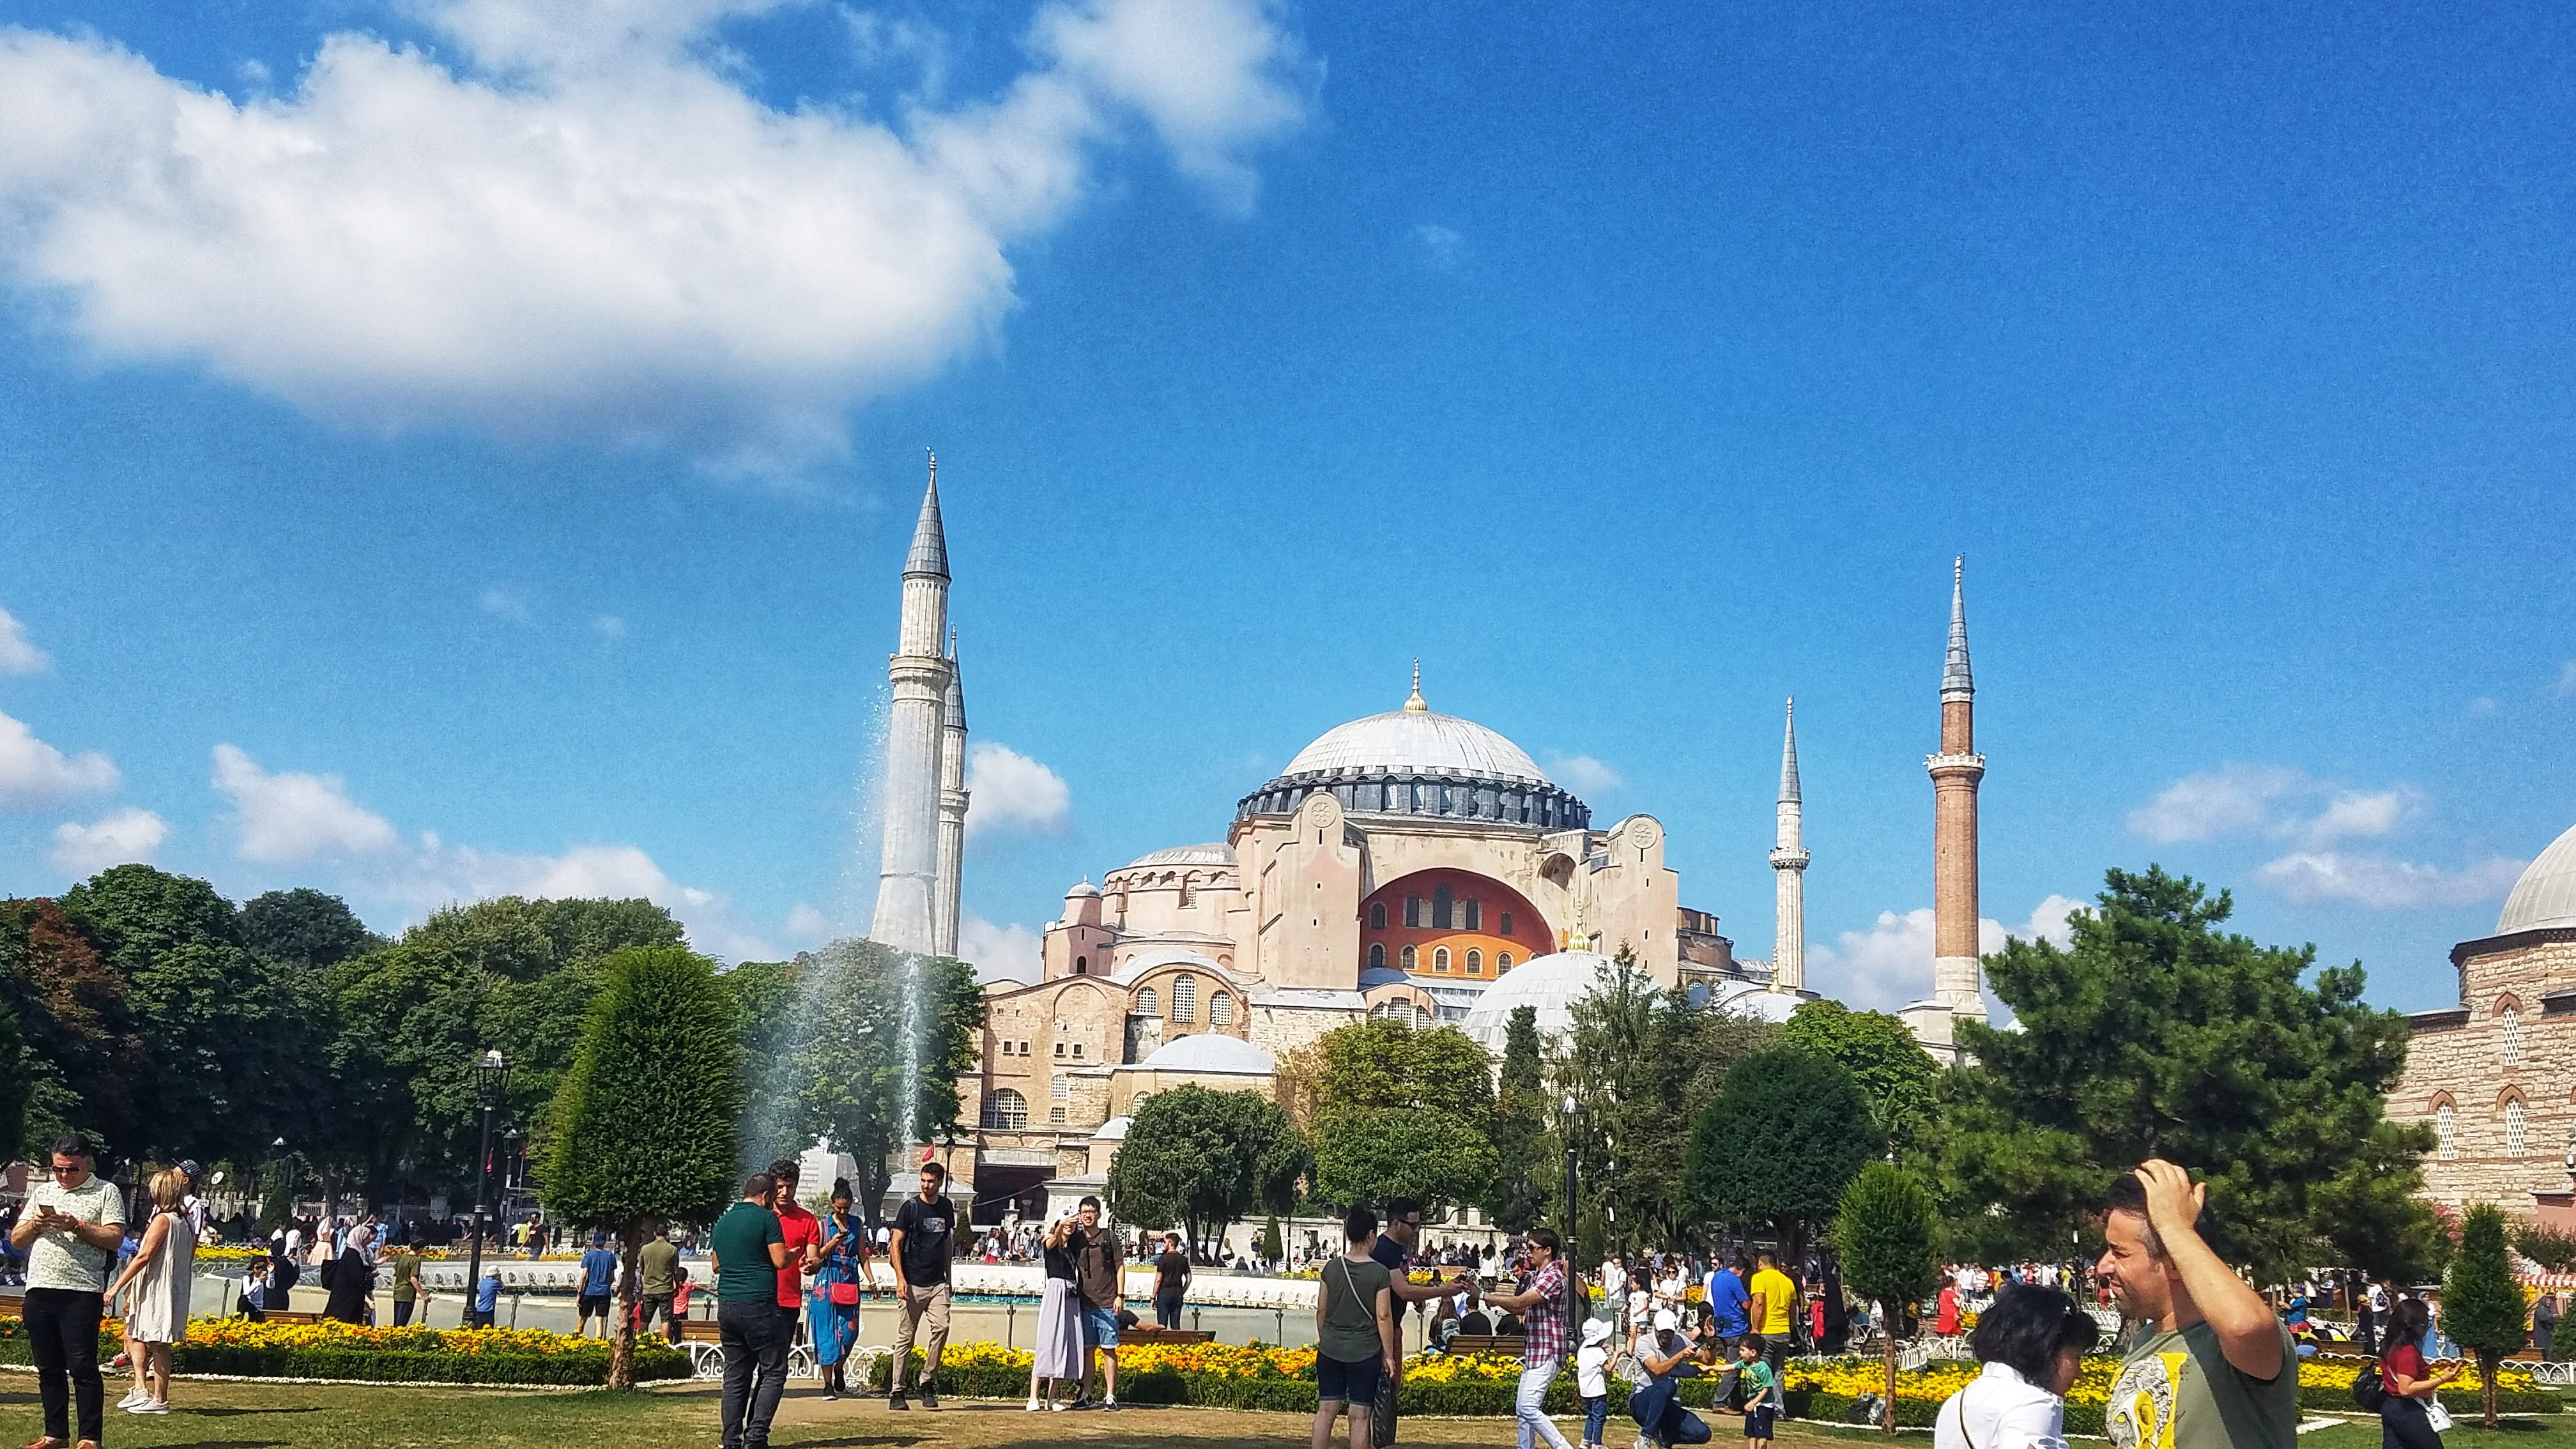
\includegraphics[width=0.7\textwidth]{img/hagia-sofia.jpg} 
%\captionsetup{justification=centering}
\caption{Hagia Sofia - wikimedia commons}
\end{figure}

The final piece included in the anthology \cite{hagan2017sound} comes from Gerriet K. Sharma and is titled \textit{mirage 4} (2015). The piece was composed with and for the icosahedral\footnote{Speaker approximating a sphere with 20 faces and one speaker for each phase of the geometry.} loudspeaker developed by the Institute of Electronic Music and Acoustics (IEM) at the aforementioned ZKM\footnote{ZKM stands for "Zentrum für Kunst und Medien" which translates to "Center for Art and Media Karlsruhe", Karlsruhe the city in Germany where the cultural center is located.}. This icosahedral speaker, takes the concept of ambisonic microphones, which capture soundfields at a single point, and invert the mechanism, attempting to project a soundfield from a single point in space, with increasing resolution based on the number of transducers. 

\cite{wendt2017perception} by Wendt, Sharma, et al. discusses the ability of such a system to reproduce accurate spatial dimensions of sound for compositional means. The system is indeed capable of creating the impression of moving trajectories of sound by exploiting wall reflections which are perceived as virtual sources. These coincident speaker arrays can be considered as a portable and affordable means for spatial music reproduction. The greatest benefit these provide, for composers, is the ability to reproduce \textit{periphonic} spatial music, that is, sound with height, without having to rely on the venues' loudspeaker array. 

Ontologically, Sharma has framed his composition using the language of sculptors, discussing at length about materiality of sound, and the treatment of space as a plastic - and malleable - medium. Unfortunately, the recording included seems to suffer from significant noises, which I don't believe were intentional. These were picked up by the binaural recording system during the recording of the piece. It is however, entirely possible that these sounds \textit{are} intentional. The predominant sounds in the work are long, noisy, and soft. The piece reminds one of an ethereal, nebulous cloud, floating above them. There is a clear motif, with identical pitches reappearing at different points of the piece together with synthesized drones. 
 
\todo[inline]{these are all from a single anthology. I will find other sources as well. There are also other spatial music works/artists I have not yet talked about. Some of them might go both in historical and new works. See macedo-2015-snd-in-space.pdf }

\subsection{Film \& Theatre}

\subsubsection{Film}
Multi-channel music is most popular in film and theatre settings. While XR devices remain relatively inaccessible for most of the world, it is common to see surround sound systems employed in movie theatres around the world. This has made formats like 5.1, and above, well-known to sound engineers, and patrons, around the world. 

% see manolas-2009-cinematic-multichannel.pdf
% see karagosian-1999-multichannel-film-sound.pdf 

\subsubsection{Theatre}

Vilkaitis and Wiggins\footnote{Bruce Wiggins's website contains a wealth of information and software for ambisonic reproduction. \href{https://www.brucewiggins.co.uk/?page_id=78}{Link.}} \cite{vilkaitis2019ambisonic} describe a case study wherein ambisonic sound design was used for a theatrical rendition of King Lear (Shakespeare). According to the authors, there are two main methods for spatial audio content creation:

\begin{enumerate}
    \item \textbf{Scene based:} with scene based spatial audio the rendering complexity is much lower. The spatial fidelity and resolution is also greater than with object based systems. The encoding and decoding are also separate, allowing one mix to be rendered in any speaker configuration, even headphones. 
    \item \textbf{Object based:} object based spatial audio is also format agnostic but works on the premise of "separating sound files into audio objects with  associated metadata describing various traits such as position and level, which are then rendered in real-time depending on the speaker layouts." The real-time rendering is more computationally taxing. 
\end{enumerate}

Scene based audio lends itself well to theatre since it already is based on scenes but object based is more flexible in that it can be edited on the fly. In contrast, scene based audio is pre-rendered, which makes quick editing impossible. It is also possible to render scene-based audio in real-time, however, this reduces the possible complexity of the sound field since the computational power becomes a bottleneck. By pre-rendering the audio scene we can add much more complexity (ie. sound sources) to the sound field. 

An important aspect of the sound design in this context is \textit{spatial unmasking}. Spatial unmasking is achieved by separating auditory events in space. This concept is related to the "cocktail party effect" which describes the ability for the auditory system to discriminate between sound sources at different locations in space. Spatial unmasking reduces the need for equalization and dynamic processing since "source separation in the spectral domain is no longer the sole method of discriminating auditory events.\cite{vilkaitis2019ambisonic}" 

In order to design the sound scenes the authors used Wiggins's ambisonic software in Reaper\footnote{\href{https://www.reaper.fm/}{Reaper} is a very popular DAW in the spatial audio community. It is not open source but there are experimental Linux builds. The large channel count per track and low cost have made it popular in the ambisonics community.}, including a 3rd order ambisonic panner and a 1st order ambisonic reverb\cite{wiggins2016ambifreeverb}. They also made use of the sound library FreeSound\footnote{https://freesound.org/} which features crowd sourced sounds from all over the world, many of which can be used commercially. In order to trigger the different sound scenes they used the markers feature in Reaper, giving it a similar functionality to QLab\footnote{https://qlab.app/}, a typical tool in theatre sound and lighting design, which unfortunately, does not support spatial audio. 

One of the main issues the authors reported, which is common for spatial audio, is the creation of a consistent experience for all patrons - in certain seats, which were close to speakers, the sound effects were too loud. One possible solution is to simply lower the volume of all the speakers, however, this could make the audio too low for the center seats. This highlights the importance of matching the audience area with the correct speaker coverage. In this case the problem was there was not enough space between the speakers and the edge seats of the auditorium. This problem could have been solved by hanging the speakers, unfortunately this is much more expensive to do safely.

Another problem was monitoring the sound scenes because the mixing desk was not centered in the auditorium. The authors suggest using a iPad with OSC to mix the ambisonic scenes wirelessly while listening from various positions. Reaper can receive OSC, as can Ardour, and many applications exist for Android and iOS that would allow one to mix from a tablet remotely. 

Upthegrove \cite{upthegrove2019auragami} recently published a MFA thesis which described the creation of several theatrical works involving spatial audio. These were created at VTech\footnote{Virginia Polytechnic Institute and State University} which hosts Cube Fest, one of the most prestigious High Density Loudspeaker Array (HDLA) concerts in America. The thesis is a good source of inspiration for artists wishing to engage with spatial sound using commercial state-of-the-art tools. Unfortunately, many of the proposed systems in this thesis are outside the reach of many artists. Some low-cost and interesting tools to highlight from this thesis include:

\begin{enumerate}
    \item \textbf{OpenAIR}: impulse response library used for convolution reverb. \href{https://openairlib.net/}{Link.}
    \item \textbf{Dante Virtual Soundcard}: a low-cost \textit{virtual} sound card which can be used in lieu of an audio interface in certain venues such as CPMC 122. \href{https://www.audinate.com/products/software/dante-virtual-soundcard?force=true}{Site.}
\end{enumerate}

% Upthegrove also makes use of some other sound design tools worth highlighting presented here in a separate list since these are not spatial audio specific: 

% \begin{enumerate}
%     \item \textbf{SFZ Players}: is a file format to define how a collection of samples are arranged for performance. Most SFZ players are free and open Source. \href{https://sfzformat.com/}{Site.}
%     \item \textbf{SPEAR}: Sinusoidal Partial Editing Analysis and Re-synthesis software. Does not work on Linux unfortunately. Pd's \texttt{partialtracer} example serves a similar purpose. \href{http://www.klingbeil.com/spear/}{Site.}
% \end{enumerate}

\subsection{Video games \& XR Experiences}
%  http://www.visual-memory.co.uk/b_resources/Munday%202007%20Music%20In%20Video%20Games.pdf

%https://en.wikibooks.org/wiki/History_of_video_games/XR

While it might seem like a departure from the world of high-art, video games have increasingly become a source of good quality musical works. Many of the most poignant examples of spatial music come from this domain. Video games often already come equipped with interactive systems which allow the player to experience 3D sound. In fact, sometimes the immersive nature of the sound is critical to the game-play - an enemy's location can be known from their footsteps ahead of time. 

In sophisticated titles, realism is an important part of the game-development process. While most of the attention and resources of the game process are often devoted to the graphics, there is definitely some care given to the music as well. Much like in film, it is important to consider both the diagetic and non-diagetic material. 

For example, in the popular titles \textit{Grand Theft Auto} (GTA) and \textit{Assassin's Creed} we encounter Role Playing Games (RPG) in which the characters encounter music in one way or another. In GTA the character can typically encounter music inside vehicles, which have tunable radios. In Assassin's Creed there are often music groups outside which perform folk music indicative of the time period. In both of these examples we can hear the panning around of the sound sources as the user moves around the scene in third person, and as we move closer and farther away, we can also experience the effect this has on the sound. In both of these cases, as in many other games, however, there is more emphasis on 3D audio for sound effects than music. 

Because there can often be hundreds of sound sources that need to be spatially represented in these titles, many authors have described strategies for dealing with the computational costs associated with this problem. In particular, one of the latest advancements and continuing areas of research in this area is a way to exploit the low cost and computational superiority of Graphics Processing Units (GPU) for audio algorithms. On a dollar-per-dollar basis, GPUs are more powerful than Central Processing Units (CPUs) \cite{hamid2009review}. Moore's Law predicted that computational speed would double every two years on average. While CPU speeds have doubled in speed every 18 months, GPUs have increased in speed by a factor of 5 during the same time. As a result, many sound engineers interested in spatial sound for video games have looked at ways to offload the computational cost of spatial audio algorithms to GPUs. Some authors have also suggested optimization algorithms based on \textit{culling} of audio sources.

General purpose GPUs allow more than just graphic rendering via programmable GPU software. The general pipeline for GPUs includes a: \textit{vertex stage}, \textit{rasterization stage}, and \textit{fragment stage}. A \textit{vertex} is simply a point, consider the cube as a simple example. The minimum number of vertices needed to represent a cube is 8. These vertices are then connected to each other via 12 \textit{edges} during the rasterization stage. Finally, the color of the cube is determined during the fragment stage, using a \textit{texture} stored in memory. The final stage is the \textit{composition stage}, during which pixel values are determined from the fragments. Languages such as \textit{OpenGL} can be used to program specific behaviors at different stages. 

\begin{figure}[ht!]%force figure here, top, strict
\centering
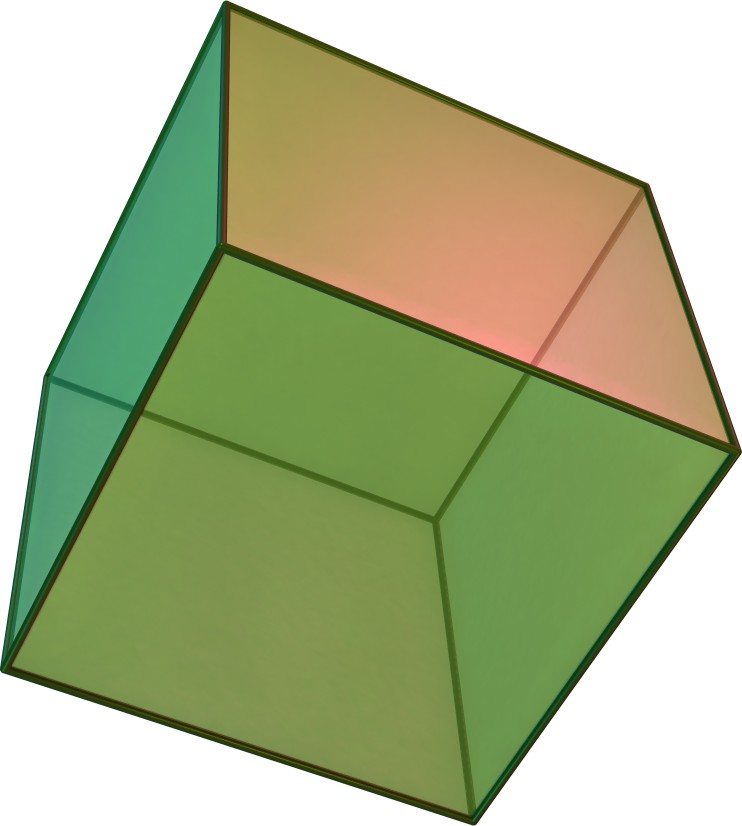
\includegraphics[width=0.5\textwidth]{img/cube.jpg} 
%\captionsetup{justification=centering}
\caption{Cube \cite{FileHexa46online}}
\label{fig:cube}
%license: This file is licensed under the Creative Commons Attribution-Share Alike 3.0 Unported license.
\end{figure}

\cite{hamid2009review} provides a review of various GPU-based sound processing algorithms. Here we will focus solely on those that can be used for spatial audio processes. As Hamid et al. note, digital signal processing (DSP) functions are suitable for GPU-based processing since they are parallelizable, arithmetically intense, have limited data dependency, and make use of multiply-add (MADD) calculations. Whalen \cite{whalen2005audio} explores using pixel shaders\footnote{A pixel shader, also known as a fragment shader, is a program that dictates the color, brightness, contrast, and other characteristics of a single pixel (fragment). A programmer who specializes is writing pixel shader programs is known as a shading artist.} for executing audio algorithms, and compares GPU to CPU performance. The authors of this study implemented some common music systems like filters and delays. Texture access, which has improved since that study, limited the performance of the filters, when compared to CPU benchmarks. 

\cite{trebien2008real} proposed a GPU-based method for real-time sound generation of multi-channel audio. For certain algorithms, the GPU showed speed-ups of up to four orders of magnitude. In other words, the GPU was more than 10,000 times faster than the CPU implementation. \cite{gallo2004efficient} considered variable delay-line and filtering algorithms, both common to spatialization, using GPUs. Delaying the signal was accomplished via texture re-sampling, while filtering was performed using a four-band equalizer. Sound signals were stored as RGBA textures where each component head a band-pass version of the original signal. 

Despite the increase performance, Gallo and Tsingos noted the shortcomings of the GPU-based implementation. Namely, long 1D textures cannot be accessed easily, and IIR filters cannot be implemented efficiently. Also, the GPU only supported 8-bit mixing, which degraded the sound quality. It should be noted that this experiment was conducted in 2004, recent developments in GPU-based spatial audio algorithms have improved performance. Just as recently as 2015, Belloch et al. \cite{belloch2014multi} showed a parallel IIR filter implementation that runs on a GPU, which was used to equalize a WFS system. The implementation ran 1256 simultaneous IIR filters of 256 samples each in real-time with a latency time of 0.72 ms.  

GPUs have also been tested in convolution operation for binaural synthesis by several authors. \cite{cowan2009real} presented a GPU-based convolution method for spatial auditory cue rendering in video games and virtual environments. The comparison showed a processing time of 2-4 ms, depending on graphics card, compared to 4-25 ms on the CPU. A range of signals of lengths spanning from 5,000 to 60,000 explains why the CPU performance varied so much. With a constant running time of 2 ms for convolution the tested video card was shown to be suitable for auralization of FX and music. 

Personalized HRTFs have been shown to improve localization, especially with regard to elevation \cite{kapralos2008virtual}. In \cite{rober2006hrtf}, Röber et al. described an alternative approach to measuring personalized HRTFs in which GPU-based ray-tracing techniques using a 3D mesh model are used to approximate HRTFs. This experiment lacked verification of the method and the diffraction effects of the head were not taken into account. \cite{sung2013individualized} recently conducted a similar experiment in which they improved the ray tracing algorithm to include diffraction at low frequencies and furthermore verified the results using objective measures. Much more recently, in 2020, Guezenoc and Séguier \cite{guezenoc2020hrtf} published a complete survey of HRTF Individualization discussing the most up-to-date work involving both four different types of HRTF individualization methods: 

\begin{enumerate}
    \item \textbf{Acoustic measurement:} acoustic method wherein impulse responses are gathered using in-ear microphones and grids of loudspeakers. 
    \item \textbf{Numerical simulation:} using 3D scans of human subjects. 3D scans can be taken using low-cost consumer grade smartphones \cite{kaneko2016deepearnet}. 
    \item \textbf{Indirect individualization based on anthropometric data:} 
    \begin{enumerate}
        \item \textbf{Adaptation:} using anthropomorphic features of the subject, a generic, or pre-existing HRTF set is modified. 
        \item \textbf{Selection:} using a data set which includes anthropomorphic information, a specific pre-measured HRTF set is selected. 
        \item \textbf{Regression:} the HRTF set is estimated using morphological measurements. A statistical approaches are used to derive the set. Some neural network approaches have been considered.
    \end{enumerate}
    \item \textbf{Indirect individualization based on perceptual feedback:} 
    \begin{enumerate}
        \item \textbf{Selection:} perceptual evaluation task is undertaken by the subject to help select the best HRTF set from the data set.
        \item \textbf{Adaption:} based on responses from subjective evaluation, a HRTF set is adapted using frequency scaling, filter-tuning, or statistical-tuning. \footnote{Refer to \cite{guezenoc2020hrtf} for more details on these three methods.} 
    \end{enumerate}
\end{enumerate}

\todo[inline]{hamidi-2009-gpu-spat-snd-review.pdf Continue 3.1. GPU-Based Acoustical Modeling - Modeling the RIR.}

\todo[inline]{Haven't talked about culling at all yet. see hacihabiboglu-2017-spat-audio-rec-sim-ren.pdf}


\section{Open Tools for Spatial Music} \label{sec:open_tools_spat_mus}
% This section will provide an overview of different existing tools for computer musicians which facilitate the creation of spatial music. We will focus on free and open source tools which work in conjunction with computer music languages such as Pd, SuperCollider, Csound, etc. 

Composers interested in working with computers are well aware of the various different ecosystems existing for the creation of computer-music works. A short list of these systems include: Puredata (Pd), SuperCollider, csound, MAX/MSP, RTcmix, and ChucK. 

In this section we will focus on Pd available tools for creation of spatial works given our familiarity with the system, as well as it's free and open-source nature. Even by focusing only on Pd, there are a slew of available tools that people have developed and published, here we will try to focus on those we find most comprehensive and well supported. 

Our motivation for using FOSS is to democratize access to art-making solutions and consider ways in which we can include as many students as possible into the spatial music-making process. While there are more sophisticated tools out there for making spatial music which one can purchase, we wanted to focus on improvements that can be made to FOSS to bring them up to par with the best commercial systems. 

\subsection{VBAP} 
Vector Based Amplitude Panning (VBAP) is an algorithm written by Ville Pulkki \cite{pulkki1997virtual}. The main drawback of this system is that there is no dedicated binaural rendering system, so it requires a collection of speakers in order to develop the works. One could use a binaural renderer such as \texttt{earplug\~} but there is no obvious way to use a head-tracker, which means the user will need access to a multi-channel sound system. 

The benefit of VBAP is that it is re-configurable to any speaker format, much like ambisonics. The added benefit of ambisonics is that the soundfield can be manipulated using a number of linear transformations which we will discuss later. VBAP is extremely simple to install and operate. 

With Pd installed, the user can simply search for the VBAP externals by typing VBAP under the "Find externals" option in \texttt{Help}. After installing, we recommend shutting down Pd and re-launching it. Make note of where Pd offers to install VBAP. It may suggest installing it inside the Pd app itself. This is a good option because it means one does not need to specify a path to the externals, Pd will automatically know where to find them. The drawback is if one installs a new version of Pd, and deletes the old, you will have to remember to download VBAP again. Alternatively, you can specify a folder of your own choosing and point Pd to it, using the \texttt{Path...} settings under preferences, or by invoking the \textit{[declare]} object in pd.

With VBAP installed now go to \texttt{Help > Browser > vbap} and open up \texttt{vbap-help.pd} to get started. Figure \ref{fig:vbap-5.0} shows an example of using VBAP for a 5.0 set-up\footnote{The example says it is 5.1 but as you can see the sub channel is missing.}. The speaker angles are specified in 2D. The \texttt{vbap} object spits out a list of gain values for each speaker in the order they were specified by the \texttt{define\_loudspeakers} message\footnote{Remember to enable as many speakers as needed under \texttt{Media > Audio Settings} by changing output channels to the desired number.}.

\begin{figure}[ht!]%force figure here, top, strict
\centering
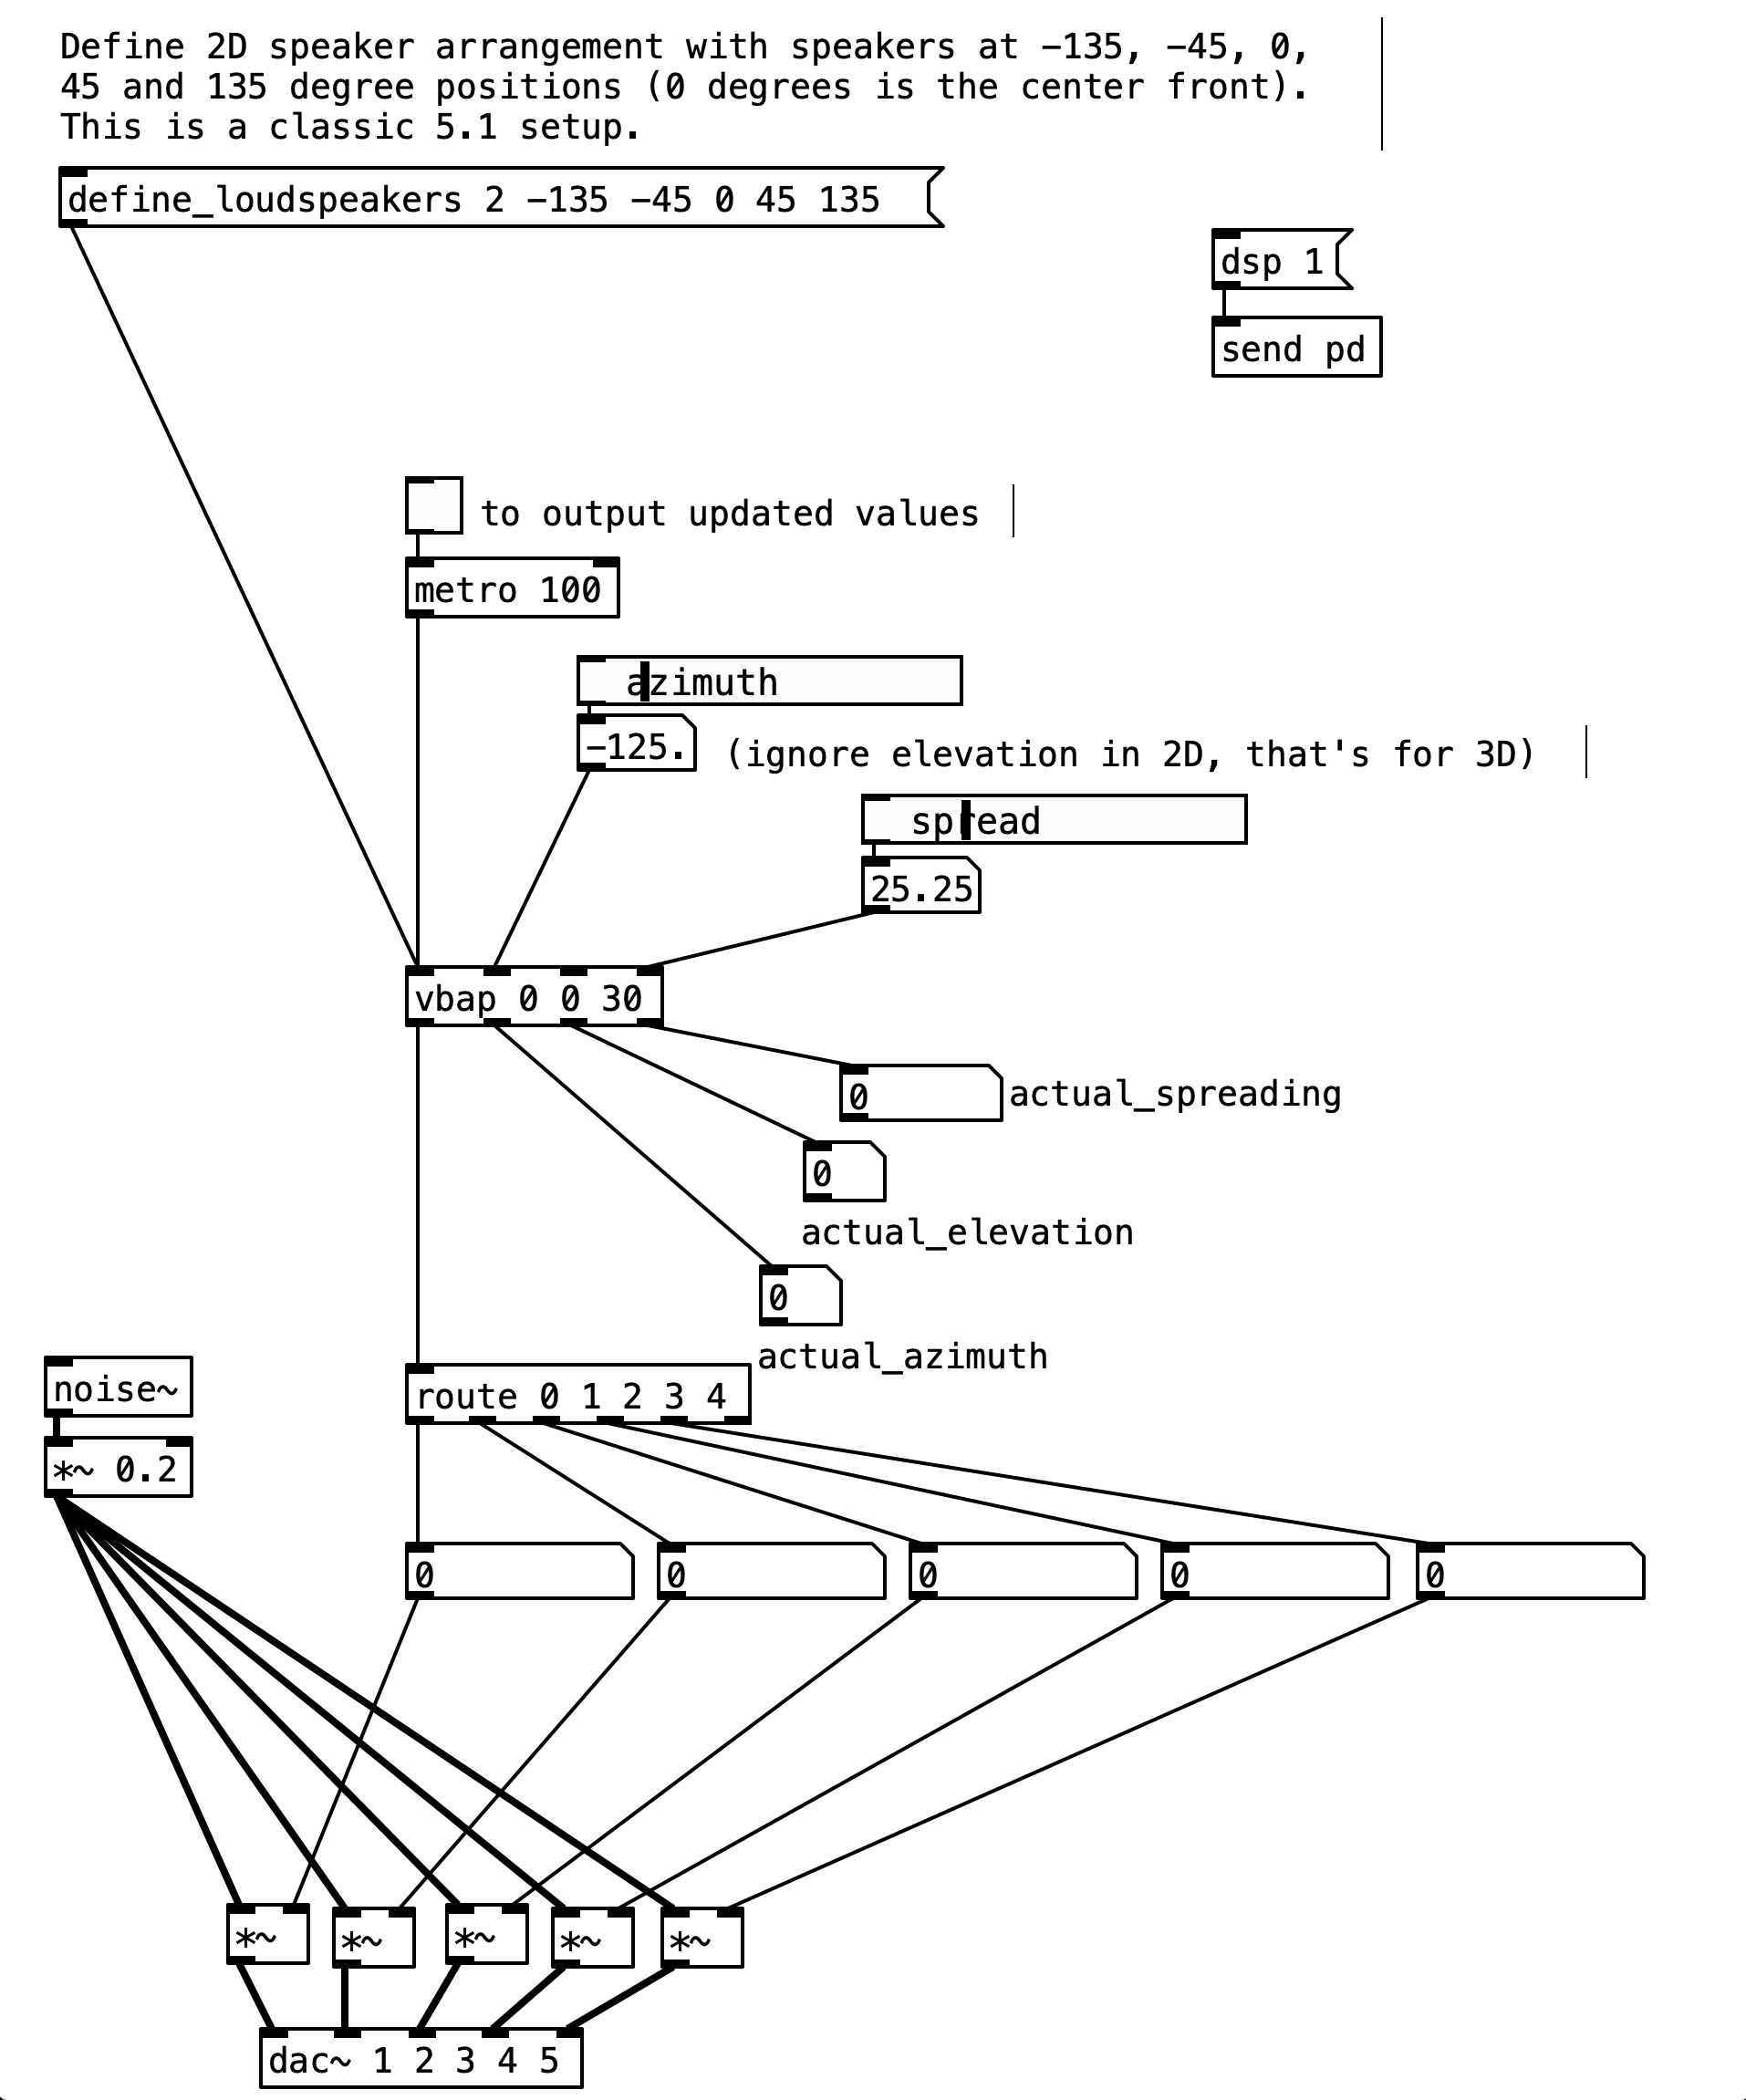
\includegraphics[width=0.7\textwidth]{img/vbap-5.1.png} 
%\captionsetup{justification=centering}
\caption{VBAP 5.0 example}
\label{fig:vbap-5.0}
%license: cc by sa 3.0
\end{figure}

In the example shown the speakers are set up in a quadraphonic arrangement with an extra speaker in the center. It does not follow the International Telecommunications Union (ITU) standard for 5.1 systems \cite{series2010multichannel} for the angles of the speakers. The ordering is also different that the standard. One has to be careful with the routing and ordering of signals, as well as angles, for good multi-channel sound reproduction. It is more common to use the ordering L/C/R/LS/RS\footnote{Left, Center, Right, Left-Surround, Right-Surround} in this format. In the example provided the order is LS/L/C/R/RS instead. 

\begin{figure}[ht!]%force figure here, top, strict
\centering
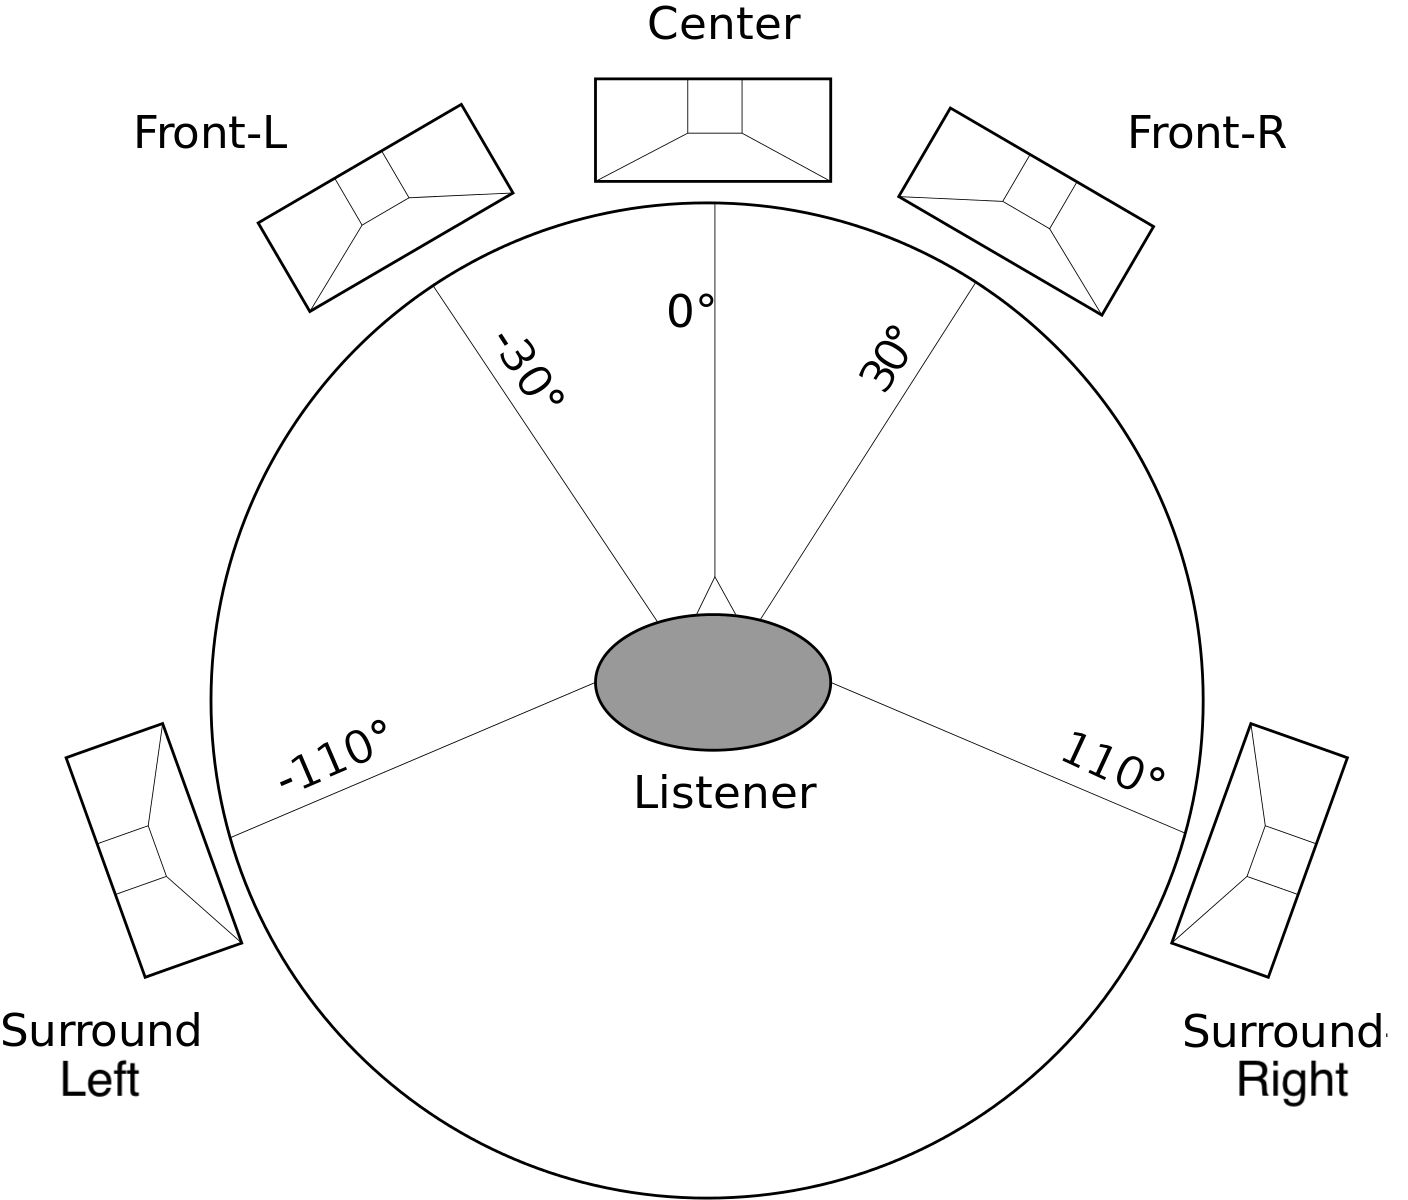
\includegraphics[width=0.5\textwidth]{img/5-1-surr.png} 
%\captionsetup{justification=centering}
\caption{ITU Standard 5.1 surround \cite{File51su81-online}}
\label{fig:5-1-itu}
%license: This file is licensed under the Creative Commons Attribution-Share Alike 3.0 Unported license.
\end{figure}

\todo[inline]{The image is cut off, I have to replace it.}

One of the main drawbacks of this is the fact that if we wanted to change from a 5.0 system to something much larger, like 22.2, we will have to manually route each gain value to its own multiply object. It is possible to use an external library with matrix operations to make things a bit simpler but for most non-experts this will likely prove too complex. Adding height is relatively simple, the message sent to the \texttt{vbap} object has to be sent a modified \texttt{define\_loudspeakers} message where the first argument is 3, which specifies 3D coordinate. The pairs of number following designate the azimuth and elevation of each speaker. 

The vbap folder also has a second abstraction called texttt{[rvbap]} which is meant to add distance effects to the signal. In our trials this external caused Pd to crash, so we recommend sticking with \texttt{[vbap]} instead and adding one's own reverb unit before the panning algorithm. This is far cheaper computationally than applying a reverb to each copy of your signal. Pd vanilla comes with 3 built-in reverb units \texttt{[rev1~]}, \texttt{[rev2~]}, and \texttt{[rev3~]}. Any one of these can be used in conjunction with VBAP to simulate distance. We recommend using a dry/wet control to dictate the simulated distance. 

\subsection{iem\_ambi}

Institute for Electronic Music and Acoustics (IEM) in Graz, Austria, has developed another useful spatialization tool for Pd. Much like VBAP this tool can also be found easily in Pd via the \texttt{Find externals} option in \texttt{Help}. Unlike, VBAP, this ambisonic toolkit is far less intuitive to operate but it does provide some improvements over VBAP. 

Perhaps the most important of these benefits is the fact that ambisonic files can be uploaded and played back over the web in scenarios where asynchronous demonstrations of spatial music are needed. The second benefit, is that a rotation on a soundfield is a linear, non-destructive, transformation which allows us to easily binaurally audition our soundfield without the need for loudspeakers. Finally, there are

\todo[inline]{According to pysiewicz-2016-spat-inst-chapter.pdf the label diffusion is specific to stereophonic sound projection and loudspeaker orchestras. However, in lynch-2017-engulfment.pdf it says "Sound diffusion refers to the practice of localizing and moving sound throughout a space using multiple loudspeakers." }


\section{Spatial Instruments}

This section will discuss the development of \textit{spatial instruments} in the 20th and 21st century. The term \textit{spatial instrument} refers to instruments which allow the user to manipulate spatial elements of sound. Spatial elements might include: direction, reverberance, width, etc. Traditional instruments generally allow the performer control over dynamics, pitch, and sometimes timbre. In contrast, \textit{spatial instrument} give the performer additional control, thus allowing the user to modify the position of sound in space whether that be for multi-channel sound reproduction or binaural synthesis\footnote{Virtual surround sound over headphones.}. 

Many instruments of this nature have been developed over the last few decades due to the popularity of multi-channel reproduction in electro-acoustic music. The development of such instruments goes back to the 1950s, with pioneering works by composers such as Pierre Schaeffer. In contrast to our common definition of instruments, many of the interfaces which will be described in this section do not produce sound at all. In fact, much of the development in Human Computer Interaction (HCI) has focused solely on the manipulation of sounds in space as separate practice from mapping controls to sound synthesis methods.  

\cite{pysiewicz2017instruments} presented a comprehensive ethnomusicological review of \textit{spatial instruments}. In that reference, the authors described a \textit{taxonomy} for the different types of spatial instruments. The five main categories from the 31 different spatialization interfaces found were: 

\begin{enumerate}
    \item \textbf{Instrument-like and augmented controllers:} simulating, inspired, or augmented with traditional/extended techniques. 
    \item \textbf{Touch controllers:} haptic/tactile interfaces.
    \item \textbf{Non-contact, extended range controllers:} free gestures in a limited sense range. 
    \item \textbf{Wearable or immersive controllers:} gloves, suits, camera tracking; performer always in sensing range.
    \item \textbf{Mixed controllers}
\end{enumerate}

Given the comprehensive work undertaken by Pysiewicz et al. we will adopt their taxonomy in our review. In addition, we will seek to integrate some examples that may be missing from the taxonomy based on research published since the aforementioned chapter was published. We strongly recommend Pysiewicz et al.'s chapter for anybody interested in spatial instrument design. In their paper, the authors further sub-divide instruments into three categories based on what spatial parameters they control. Given the ambiguity of these categorizations we have opted not to make such distinctions. One further classification however did seem useful: exclusive spatial control versus hybrid instruments featuring \textit{spatial-synthesis} \footnote{This categorization can be hard to demarcate. In general if one can entirely separate the composition process from the spatialization process, we could argue that the apparatus used for the diffusion of sound does not conform to our spatial-synthesis label.}. We will attempt to highlight spatial-synthesis instruments as we believe these constitute a more interesting family of instruments, rich with creative design possibilities for computer musicians.

\subsection{Instrument-like and Augmented Controllers}

This category refers to instruments which resemble typical musical instruments extended via the use of additional sensors. In this category Pysiewicz et al. only point out two instruments: 

\begin{enumerate}
    \item \textbf{DJ Spat:} by Marentakis et al. (2007) which extends the turntable by using motion-tracking sensors and haptic controls. The angular displacement of the performer's hand is mapped to the sound source position reproduced through a circular loudspeaker array. 
    \item \textbf{Radiodrum:} by Ness et al. (2011), is an instrument used exclusively for spatialization inspired by the radiodrum developed at Bell Laboratories in the 80's. The radiodrum uses capacitive sensing to report the position of two batons in 3D space, as well as velocity when in percussion mode. It is also known as a \textit{radio baton.} Figure \ref{fig:baton} shows Max Matthews, one of the most important figures in computer music, holding a Radio Baton.
\end{enumerate}

\begin{figure}[ht!]%force figure here, top, strict
\centering
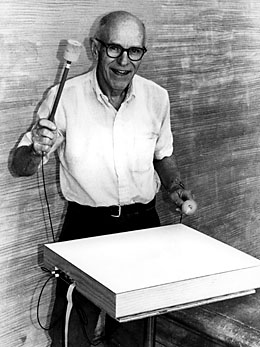
\includegraphics[width=0.5\textwidth]{img/mathews260.jpg} 
%\captionsetup{justification=centering}
\caption{Matthews waving Radio-Baton \cite{FileMath82online}}
\label{fig:baton}
%license: public domain
\end{figure}

Graham \cite{graham2014gesture} presented in 2014 an extended guitar with hexaphonic pick-ups\footnote{A special pick-up for electric guitar with discrete outputs for each string.} which uses a boids algorithm to spatialize sounds. The boids algorithm, developed by CW Reynolds, simulates the motion of flocks of birds. The discrete channels of the guitar output are also analyzed in Pd. Finally, the system includes the use of a Microsoft Xbox Kinect sensor, an infrared depth-sending device, which tracks the guitarists body.

Werner \cite{wernerdevelopment} also published some literature on a similar project entitled GASP or Guitars with Ambisonics Spatial Performance in 2020. This project, from the University of Derby, supervised by Bruce Wiggins, does not use a kinect, but relies only on a MIDI footswitch controller and a hexaphonic pick-up (either the Ubertar hex passive pick-ups\footnote{http://www.ubertar.com/hexaphonic/} or the Cycfi Nu-Series\footnote{https://www.cycfi.com/projects/nu-series/}). One noteworthy element is the creation of a "Guitarpeggiator" which was implemented using gate switching. This allows the guitarist to play arpeggios on the guitar by simply strumming a chord. 

Werner also notes that a cheaper version of this project, not relying on hexaphonic pickups, could be achieved using some frequency splitting\footnote{This might work in harmonic sections, but is unlikely to work in melodic phrasing. This is because the frequency range of individual each string might not cover the entire audible spectrum.}. The author's future work includes integrating the entire system into a single application. Currently it relies on mostly FOSS, with the except of the DAWs for ambisonic processing and MIDI event triggering (for the arpeggiation). 

\subsection{Touch Controllers} %haptic/tactile

This category refers to instruments which need to be physically interacted with, in a tactile fashion, for operation. This can include touch screen like those found in tablets or something simpler like a potentiometer or button. Same of the earliest examples of spatial instruments made use of tactile interfaces, thus, a number of historical examples will be present in this section. Below we provide a list of some of the most noteworthy examples from \cite{pysiewicz2017instruments}.

\begin{enumerate}
    \item \textbf{Sal Mar Construction:} designed in the early 1970s by composer Salvatore Martirano (USA), the instrument is a analog/digital composition machine which featured 24 spatialized audio channels. Figure \ref{fig:sal-mar} depicts the instrument (photo courtesy of the University of Illinois).
    
    \item \textbf{Hybrid IV:} developed by Edward Kobrin\footnote{Very little information could be found online about Kobrin. \cite{kobrin1968solution} suggests he was American, since this work was conducted at Northwestern University, Evanston, Illinois.} in 1975, the systems sound-making components are analog but the score is composed using digital means. The multi-channel matrix provides 16 outputs. 
    
    \item \textbf{SSSP Sound Distribution System:} developed by Guy Fedorkow et al. in the late 70s at the University of Toronto, Ontario, Canada. In contrast to the two previous examples the system was modular in nature: the polyphonic sounds are synthesized by one module and controlled spatially by another. It also featured a keyboard, tablet, and 16 outputs. 
\end{enumerate}

\begin{figure}[ht!]%force figure here, top, strict
\centering
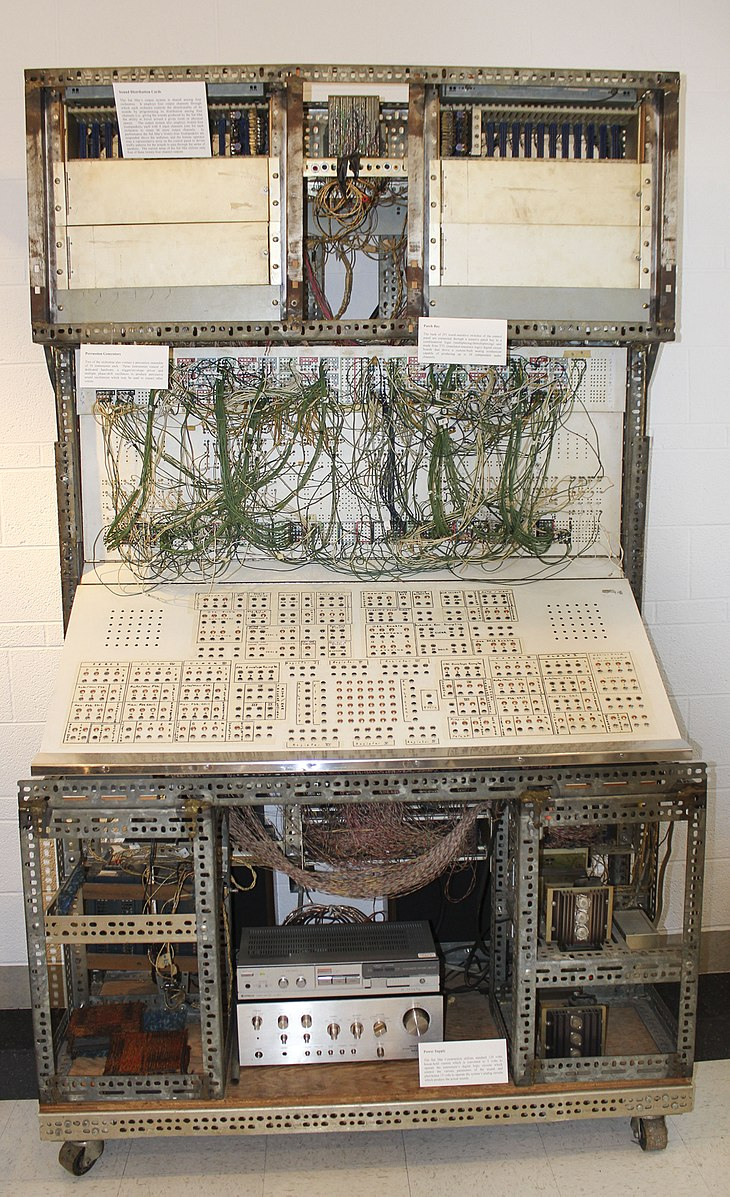
\includegraphics[width=0.5\textwidth]{img/sal-mar.jpg} 
%\captionsetup{justification=centering}
\caption{Sal Mar Construction \cite{FileTheS26online}}
\label{fig:sal-mar}
%license: This file is licensed under the Creative Commons Attribution 2.0 Generic license.	
\end{figure}

All three of these examples fall under the spatial-synthesis category, wherein synthesis and spatial control are integrated into a single instrument. The following examples are of instruments used exclusively for the spatial control of sound.

% \todo[inline]{Don't exclude anything, but you don't need details on all the systems.}

\begin{enumerate}

    \item \textbf{HaLaPhon:} invented in the late 1960s by Hans-Peter Haller and Peter Laszlo, the instrument counted with switches and automation for the control of sound diffusion in circular arrangements by employing amplitude panning. The device evolved from analog to digital versions, all maintaining the overall concept.
    
    \item \textbf{Loudspeaker Orchestras:} there are multiple Loudspeaker Orchestras such as the Gmebaphone (1973) (also known as the Cybernephone), the Acousmonium (1974), and the BEAST System (1986). These all share portability as a key feature and an associated fader board system for spatialization. These instruments were developed at Bourges\footnote{France.}, Paris, and Birmingham respectively. The speaker arrangements are very specific, in contrast to other systems.
    
    \todo[inline]{Detail missing here. Composers. Pieces. Loudspeaker Orchestras is huge topic. There is a bit of overlap w/ Ch2 section on electro-acoustic music, try to not repeat yourself, cross-reference instead.}
    
    %% Don't exclude anything, but you don't need details on all the systems. I will make a small list of the things I leave out intentionally.
    
    % \item \textbf{TRAILS:} the Tempo Reale Audio Interactive Location System was created by Bernardini in 1989. It does not define specific speaker layouts.
    
    \item \textbf{Rotation Mill (Tonmühle:} was conceptualized in the 60's at the Technical University of Berlin and later used by Karlheinz Stockhausen for use at the Osaka World Expo in 1970. At the expo the rotational resistance device was patched to 50 loudspeakers surrounding the audience.
    
    %\item \textbf{Circular Relay Switch:} Leitner in 1971 %is this same as bernard leitner from installation works?
    
    \item \textbf{Spherical Sound Controller:} was also designed for the 1970 World Expo, this time for use in the West German pavilion. It was also created by the Electronic Music Studio at the Technically University of Berlin and "consisted of 50 sensor buttons, each representing a loudspeaker group in the spherical concert hall" \cite{pysiewicz2017instruments}. The instrument allowed sources to be projected and moved in space.
    
    %\item \textbf{MusicSpace}
    
    \item \textbf{Expanded Instrument System:} or EIS, for short, was developed by Pauline Oliveiros starting in 1963. It constitutes a performance environment that "intends to give performer control over the acoustic space" \cite{pysiewicz2017instruments}. EIS features: amplitude panning, delays, and a reverb unit, connected to an interface consisting of several footswitches.
    
\end{enumerate}

The above list constitutes some historical examples of tactile interfaces for sound spatialization. Below we will continue with the category focusing on technologies developed in the 21st century\footnote{For sake brevity a few instruments have been left out of our list such as the: \textbf{TRAILS} (Bernardini 1989), \textbf{Circular Relay Switch} (Leitner 1971), and \textbf{MusicSpace} (Pachet and Delerue in 1999).}.

\begin{enumerate}

    \item \textbf{M2:} was created by Mooney in 2004 and presented as a modular diffusion system featuring digital rendering engine and a specifically designed fader board. The system allows for grouping of sound sources which could be a useful feature in these systems. For example one might group all percussive elements together and use a single fader to control their volume.
    
    \item \textbf{Multi-Touch Soundscape Renderer:} \cite{bredies2008multi} was created by Bredies et al. in 2008 and comprises of a multi-touch tabletop used for manipulation of sound objects rendered using WFS via a circular array of speakers. One of the noteworthy elements of this project is the ability for multiple people to interact with the tabletop at once. This particular tabletop was based on the Frustrated Total Internal Reflection (FTIR) technique \cite{han2005low}. The tabletop was built as a testing environment for the Soundscape Renderer\footnote{http://spatialaudio.net/ssr/} (SSR).
    
    \todo[inline]{reactable, audiopad, LEMUR, ISS Cube, Audiocube, IOSONO all in bredies2008multi (bibtex) } 
    
    \todo[inline]{johnson-2014-diffusing-diffusion.pdf}
    
    \item \textbf{Tactile.space:} is another similar project by Johnson and Kapur (2013) which was later expanded into a tablet-based system making it more portable and personalized. The \textbf{tactile.motion} tablet application uses amplitude panning sent via OSC to a main computer for sound spatialization. 
    
    \item \textbf{Sound Surfing Network:} is another mobile spatialization application this time presented by Park et al. (2013). The system is comprised of two cell-phone apps, one for the performer and one for the audience. The audience app "turns each smartphone into an element of the loudspeaker array" \cite{pysiewicz2017instruments}. Unfortunately, cell-phone speakers do not have particularly good frequency response. However, if these small cell-phone speakers were supplemented with an additional pair of bigger speakers, capable of reproducing some of the missing "low-end", this might be a noteworthy experience.
    
    \item \textbf{Sound Flinger:} is a haptic controller for spatial-synthesis control of sound. It was created in 2011 by Carlson et al. This simple design uses just two buttons and four faders to control a physical model in a quadraphonic system. The physical models are accomplished via Edgar Berdahl’s haptic object library \cite{berdahl2010hsp} and runs on a Beagleboard\footnote{https://beagleboard.org/} using a PlanetCCRMA distro\cite{lopez2005surviving}. From an informal survey, users reported the need for the instrument to have a visual representation of sound sources, in order to facilitate playing sounds in space.
    
\end{enumerate}

\subsection{Non-contact, Extended Range Controllers} %free gestures

This section corresponds to instruments which require to physical touch for their operation. This includes systems using either light sensitive receivers or electromagnetic sensors (aka. inductive capacitance). 

\begin{enumerate}
    \item \textbf{Photocell Mixer:} was developed in the 1960s by Frederic Rzewski (1968) and David Behrman (1967). Each composer developed their photocell mixer independently but they both shared the same principles. Panels with photocells are integrated into the signal circuit. Using a penlight, the user can assign signals to loudspeakers by reducing the resistance between components separated by the photoresistors\footnote{A photoresistor is a passive component that decreases resistance with respect to receiving luminosity on the component's sensitive surface.}. 
    
    \item \textbf{Light-Emitting Pen Controller:} was developed by Brown et al. in 2005. In their approach light-emitting pens are captured and tracked in space using computer vision algorithms. Their particular implementation made use of the Jitter visual programming environment included with Cycling 74's MAX/MSP\footnote{https://cycling74.com/products/max/}. 
    
    \item \textbf{Grainstick:} was created by Leslie et al. at IRCAM in 2010 and shows a multi-modal approach to controller systems which employs both infrared motion tracking and accelerometer data. Each grainstick has a number of reflective balls which can be tracked by the infrared sensors in space. The data from both the infrared capture and the accelerometer (from the Wiimote) is used to drive a granular synthesis system using WFS. The synthesis is accomplished using the CataRT Library for MAX/MSP \footnote{http://ismm.ircam.fr/catart/}. There is also some gesture analysis applied to the accelerometer data via the Jamoma\footnote{http://www.jamoma.org/} framework. This instrument also fits within our spatial-synthesis category since each grainstick controls both spatialization and synthesis parameters.
    
    \item \textbf{Pupitre d'Espace:} is perhaps the oldest of all the instruments in our list. It was developed by Pierre Schaeffer in 1952 and operated on the basis of electromagnetic inductance. Four induction coils are mounted around the performer as receiver rings. One additional coil is held in the hand of the performer. The distance between the receiver rings and the moving coil in the performer's hand induces four currents which are used to control the amplitude of four speakers. 
    
    \item \textbf{NAISA:}
    \item \textbf{Gesture Controller for a WFS System}:
    
    \item \textbf{Holistic Spatialisation System for Multiple Sound Sources:} (HSSMSS) is a controller presented by Diatkine et al. in 2015, which makes use of a "short-range infrared sensor" capable of tracking hand gestures and mapping these to musical parameters. The system relies on HOA for the spatialization of sound sources, a LeapMotion\footnote{https://developer.leapmotion.com/} controller, and MAX/MSP as the main environment. It also supports binaural synthesis with head-tracking for auditioning of sound-fields via the \texttt{Sarcoder\~} MAX/MSP external.
\end{enumerate}

\subsection{Wearables or Immersive Controllers} %always in sensing range


\subsection{Mixed Controllers} %no definition


\subsection{VRMIs}
\todo[inline]{For now I am using a separate category. I have to go back and integrate.}

Virtual Reality Musical Instruments (VRMI) (serafin-2016-vr-inst.pdf) constitute a new type of musical instrument that include simulated visual data shown using a HMD or CAVE system. Serafin et al. hypothesize two reasons why perhaps these instruments have been paid less attention:

\begin{enumerate}
    \item Musicians generally rely on sound and touch for performing on their instruments.
    \item Devices providing visual feedback that are both low-cost and portable have only recently become available (ie. Oculus HMDs). 
\end{enumerate}

VRMIs, according to the authors, is limited to visual feedback via an immersive system. In other words, 2D projection of 3D environments is not considered sufficient for an instrument to be considered a VRMI. These multi-modal virtual musical instruments (VMI) are also interesting and often spatial, but not part of a true VR system.

One of the challenging aspects of these instruments is that it is hard for the audience to witness the performance, since the musician is donning a HMD offering a personalized experience. It is possible to project a \textit{monoscopic} view of the performers action, however, the discourse between musician and audience will be lost, to some extent, as the performer will have no sense of his or her surroundings. 

\begin{enumerate}
    \item \textbf{CORDIS-ANIMA:} (Cadoz et al. 1993) this system has never been strictly used as a VRMI but it has all the elements necessary to create a sophisticated VRMI. Namely, it features physical models for both auditory and visual phenomena. 
    
    \item \textbf{}
    
\end{enumerate}

In addition to providing a survey of some VRMIs, Serafin et al. (serafin-2016-vr-inst.pdf) also provide some guiding principles for VRMI design. 

%%%%%%%%%%%%%%%%%%%%%%%%%%%%%%%%%%%%%%%%%%%%%
\section{Open Tools for Spatial Instruments}

\section{The Future of Spatial Music \& Instruments}

\section{Conclusion}



